\documentclass[11pt]{article}
\usepackage{amssymb}
\usepackage{latexsym}
\usepackage{amsmath}
\usepackage{amsthm}
\usepackage{mathtools}
\usepackage{natbib}
\usepackage{tikz-cd}
\usepackage{stmaryrd}
\usepackage{MnSymbol}
\usepackage{geometry}
\usepackage{enumitem} 
\usepackage{hyperref}
\usepackage{bbm}
\hypersetup{
    colorlinks,
    citecolor=blue,
    filecolor=red,
    linkcolor=blue,
    urlcolor=blue
}
\newtheorem{thm}{Theorem}[section]
\newtheorem{prop}[thm]{Proposition}
\newtheorem{lemma}[thm]{Lemma}
\newtheorem{exercise}[thm]{Exercise}
\newtheorem{cor}[thm]{Corollary}
\newtheorem{dfn}[thm]{Definition}
\newtheorem{axiom}[thm]{Axiom}
\newtheorem{rmk}[thm]{Remark}
\newtheorem{ex}[thm]{Example}
\newtheorem{question}[thm]{Question}
\newtheorem{problem}[thm]{Problem}
\renewcommand{\baselinestretch}{1.05}
\newcommand{\pd}{\partial}
\newcommand{\reals}{\mathbb R}
\newcommand{\cplx}{\mathbb C}
\newcommand{\intg}{\mathbb Z}
\newcommand{\bbf}{\mathbb F}
\newcommand{\bbk}{\mathbb K}
\newcommand{\ratl}{\mathbb Q}
\newcommand{\torus}{\mathbb T}
\newcommand{\sca}{{\mathfrak a}}
\newcommand{\scb}{{\mathfrak b}}
\newcommand{\scc}{{\mathfrak c}}
\newcommand{\scm}{{\mathfrak m}}
\newcommand{\scn}{{\mathfrak n}}
\newcommand{\scp}{{\mathfrak p}}
\newcommand{\frakg}{{\mathfrak g}}
\newcommand{\frakd}{{\mathfrak D}}
\newcommand{\calf}{{\cal F}}
\newcommand{\calg}{{\cal G}}
\newcommand{\cala}{{\cal A}}
\newcommand{\calb}{{\cal B}}
\newcommand{\calc}{{\cal C}}
\newcommand{\cale}{{\cal E}}
\newcommand{\cali}{{\cal I}}
\newcommand{\calj}{{\cal J}}
\newcommand{\calk}{{\cal K}}
\newcommand{\call}{{\cal L}}
\newcommand{\caln}{{\cal N}}
\newcommand{\calo}{{\cal O}}
\newcommand{\calr}{{\cal R}}
\newcommand{\mathbold}{\bf}
\newcommand{\cinf}{C^{\infty}}
\newcommand{\row}[2]{#1_1,\dots ,#1_{#2}}
\newcommand{\dbyd}[2]{{\pd #1\over\pd #2}}
\newcommand{\Space}{{\bf Space}}
\newcommand{\alg}{{\mathbold Alg}}
\newcommand{\notsubset}{\not \subset}
\newcommand{\notsupset}{\not \supset}
\newcommand{\pois}{{\mathbold Pois}}
\newcommand{\pitilde}{\tilde{\pi}}
\renewcommand{\qedsymbol}{$\square$}
\newcommand{\rta}{\rightarrow}
\newcommand{\Lrta}{\Longrightarrow}
\newcommand{\lrta}{\longrightarrow}
\newcommand{\Llta}{\Longleftarrow}
\newcommand{\lgl}{\langle}
\newcommand{\rgl}{\rangle}
\newcommand{\inj}{\hookrightarrow}
\bibliographystyle{plain}
\title{\bf Notes for Differential Galois Theory by P. Jossen}
\author{Texed by Lin-Da Xiao} %\thanks{Research partially supported by NSF Grant DMS-96-25122 and the Miller Institute for Basic Research in Science.}
\begin{document}
\maketitle
\tableofcontents
\newpage
\section*{About the Course}
Classical Galois theory:
\begin{itemize}
\item Fields $\calk$
\item 
 Fields extensions $\calk'/\calk$.
 \item 
$Gal(\calk'/\calk)= Aut_\calk(\calk')$.
\item
Solution of polynomials, $\calk'$=``$\calk$(solutions of polynomials)'', which is what we call \textbf{splitting field}.
\end{itemize}
 
\noindent In the Differential setting, 
\begin{itemize}
\item Fields $\calk$ with derivation $\pd$, e.g. $\ratl(t)$, with usual derivative:
\item Differential field extension $\calk'\calk$
\item $Gal(\calk'/\calk)=Aut_{(\calk,\pd)}(\calk',\pd)$
\item Solution of differential equations. $\calk'=``\calk(\text{solution of differential equation})''$, which is called \textbf{Picard-Vessiot Field}
\end{itemize}

\section{Differential rings and modules}
Convention: Ring= commutative ring with unit.
\begin{dfn}
Let $\calr$ be a ring. A \textbf{derivation} on  $\calr$ is a map $\pd:\calr \rightarrow \calr$ s.t.
\begin{enumerate}
\item $\pd (a+b)=\pd a+\pd b$,
\item $\pd(ab)=a\pd b+b\pd a$.
\end{enumerate}
then we call $(\calr,\pd)$ a differential ring.
A morphism of diff-rings $\varphi:(\calr_1,\pd_1 )\rightarrow (\calr_2,\pd_2)$ is a ring morphism s.t. $\pd_2\varphi=\varphi\pd_1$
\end{dfn} 
\begin{ex}
$\ratl(t),\calk(t)$ with usual derivations and $\ratl[t],\calk[t]$, $C^\infty([0,1])$
\end{ex}

\begin{dfn}
Let $(\calr, \pd)$ be a diff-ring, Call $\calc\subset\calr$ \textbf{constant} it $\pd c=0,\forall c\in \calc$.
\end{dfn}

\begin{prop}
Let $\calc\subset\calr$ be the set of constant elements.
\begin{enumerate}
\item $\calc$ is a subring,
\item If $\calr$ is a field, then so is $\calc$
\end{enumerate}
\end{prop}
\begin{proof}
$1\in\calc$, $\pd 1=\pd (1\cdot 1)=2\pd 1\Longrightarrow \pd c=0$\\
$a,b\in \calc\Longrightarrow a+b\in \calc$, and $ab\in\calc$ by Leibnitz rule.\\
Suppose $\calr$ is a field ,$c\in \calc, c\neq 0, 0=\pd 1=\pd (c\cdot c^{-1})=c\pd (c^{-1})\Longrightarrow \pd c^{-1}=0$
\end{proof}
\begin{ex}
Caution: $\calr=\bbf_p[t]$, $\pd$ is the usual derivative. Here, constant $\calc= \bbf_p[t^p]\supsetneqq \bbf_p$, because
$$
\pd(a_0+a_1 t^p+a_2 t^{2p}+...+a_n t^{np})=0.
$$
\end{ex}

\begin{exercise}
Show that $\calc \subseteq \calr$ is a algebraically closed in $\calr$. i.e. $x\in \calr$ algebraic over $\calc$ $\Longrightarrow$ $x\in \calc$. (Notice it does not mean $\calc=\overline{\calc}$ in general)
\end{exercise}

\begin{exercise}\label{exr:1.7}
Show that for differential field $\calk$ with constants $\calc$, consider a field extension $\calr/\calk$, an element $x\in \calr$ satisfying $x'=0\in \calk$  is algebraic over $\calk\Lrta x$ is algebraic over $\calc$.\\
\textbf{Solution}:\\
$x$ is algebraic over $\calk$ , consider the minimal monic polynomial $p(X)= X^n+...a_0$ with coefficients in $\calk$. Then $p(c)=0\Lrta p(x)'=(a_{n-1}')x^{n-1}+...+(a_0')=0$ by the minimality of $p(X)$, we conclude that we conclude that each $a_{i}'=0$, thus finished the proof.
\end{exercise}

\begin{dfn}
A \textbf{differential $(\calr, \pd)$-module} $(M,\pd)$ is a $\calr$-module  $M$ , together with $\pd: M\rightarrow M $ satisfying:
\begin{enumerate}
\item $\pd(m+n)=\pd m+\pd n$
\item $\pd_M(a m)=\pd_\calr a \cdot m+a\cdot \pd_M m$.
\end{enumerate}
Think of $(M,\pd)$ as a differential equation, with solutions $ker(\pd :M\rightarrow M).$
\end{dfn}
Suppose $\calr=\calk$ is a field (over that $M$ is free), $M $ has finite dimension.
Choose a $\calk$-basis , $(e_1,...,e_n)$ of $M$.
Set
$$
\pd e_i=-\sum_{j=1}^n a_{ij} e_j,
$$
where $A=(a_{ij})\in  M_{n \times n}(\calk)$. 
The matrix $A$ characterizes $\pd :M\rightarrow M$, uniquely, by additivity and Leibnitz:
$$
m\in M, m=\sum_{i=1}^n \lambda_i e_i,
$$

$$
\begin{aligned}
\pd m & =\sum \pd (\lambda_i e_i)=\sum (\pd \lambda_i)e_i+\sum \lambda_i \pd e_i\\
&=\sum(\pd \lambda_i) e_i-\sum \sum \lambda_i a_{ij} e_j.
\end{aligned}
$$
The differential equation corresponding to $(M,\pd)$ is  the equation
$$
u'=A u.
$$
\begin{rmk}
the matrix $A$ depends on the choice of the $\calk$-basis of $M$. Choosing a different basis yields an equation $u'=\tilde{A}u$ with $\tilde{A}=S^{-1}A S-S^{-1}S'$, where $S\in GL_n(\calk)$ is the base change matrix. we called $A,\tilde{A}$ equivalent
\end{rmk}
\begin{rmk}
Let $M$ be a differential $\calk$-module, $\calc\subset \calk$ be the set of constants, then we have
$
\pd  :M\rightarrow M.
$ 
is $\calc$-linear, follows from Leibnitz.
In particular $ker \pd\subseteq M$ is a $\calc$-module (vector space)
\end{rmk}

\begin{lemma}\label{lem:basis}
Let $u'=A u$ be a differential equation with $A\in M_{n\times n}(\calk)$. Let $v_1,...,v_r\in \calk^n$ be solutions, i.e. $v_i'=A v_i$. If $v_1,...,v_r$ are linear dependent over $\calk$, then they are linear dependent over $\calc$. In particular,
$$
dim_{\calc}(\ker \pd)\leq n.
$$
\end{lemma}
\begin{proof}
Induction on $r$. For $r=1$, trivial. Fix $r\geq 2$, suppose lemma holds for $<r$ solutions. Suppose w.l.o.g that no proper subset of $\{v_1,...,v_r\}$ is linear dependent over $\calk$. We find that there is a unique linear dependence relation 
$$
v_1=\sum_{i=2}^r b_i v_i,\ b_i\in \calk
$$
$$
\begin{aligned}
0=v_1'-A v_1&=\sum b_i'v_i+b_i v_i' -\sum_{i=2}^r b_i A v_i\\
& =\sum^r_{i=2}b_i' v_i+\sum_{i=2}^r b_i(v_i'-A v_i)=\sum_{i=2}
^r b_i' v_i
\end{aligned}
$$
so $b_i'=0$ for $i=2,...,r\Longrightarrow b_i\in\calc$, and $v_1,...,v_r$ linear dependent over $\calc$.
\end{proof}
Compactify the notation , $v_1,...,v_r$ columns of a matrix $V\in M_{n\times r}(\calk)$, then $v_i'=A v_i\Longrightarrow V'=A V$. Know that $rank_\calc V\leq n$.
What we usually seek is a $V\in GL_n(\calk)$ with $V'=A V$. The columns of such $V $ provide a basis of the solution space of the differential equation and thus also a basis of the differential module itself.

\begin{dfn}
$\calk$ is a diff-field, $A\in M_{n\times n}(\calk)$, let $\calr$ be a differential $\calk$-algebra, which means we have a diff-ring morphism from $(\calr,\pd_\calr)$ to $(\calk,\pd_\calk)$. We also suppose $\calr$ has same constants as $\calk$ (every constant of $\calr$ lies in $\calk$).
A matrix $V\in GL_n(\calr)$ is said to be a \textbf{fundamental matrix} of solutions of the differential equation $u'=A u$, if $V'=A V$.
\end{dfn}
\begin{rmk}\label{rmk:fundamental_matrix}
Let $V,\tilde{V}$ be fundamental matrices of solutions of $u'=A u$, $V,\tilde{V}\in GL_{n}(\calr)$, $\tilde{V} =V\cdot S$ $S=V^{-1} \tilde{V}$
$$
A\tilde{V}=\tilde{V}'=(VS)'=V'S+V S'=A V S+V S'=A \tilde{V}+V S'
$$
$
\Longrightarrow V S'=0,
$
$V$ is invertible $\Longrightarrow S'=0\Longrightarrow S\in GL_n(C)$.
\end{rmk}

\begin{dfn}
Let $v_1,...,v_n\in \calk$, The \textbf{Wronski matrix} of $\underline{v}\in \calk^n$
is 
$$
Wr(\underline{v})=
\begin{pmatrix}
v_1  & v_2 & \cdots & v_n\\
v_1^{(1)} & v_2^{(1)} & \cdots & v_n^{(1)}\\
\vdots  & \vdots & \ddots & \vdots \\
v_1^{(n-1)} & v_2^{(n-1)} & \cdots & v_n^{(n-1)}
\end{pmatrix}
$$
the \textbf{Wronskian} is the determinant of the Wronski matrix, i.e. $det(Wr(\underline{v}))=:wr(\underline{v})$.
\end{dfn}

\section{Picard-Vessiot extension}

Through out this section, we will assume 
$\calk$ is a differential field with $char(\calk)=0$(It contains $\ratl$ as subfield). The set of constants $\calc\subset \calk$ is a field and we assume it to be algebraic closed.  For example, think of $\calk=\cplx(t),\pd=d/dt$ and $\calc=\cplx$.

\begin{dfn}
Let $\calr$ be a diff. $\calk$-algebra. An ideal $I\subset \calr$ is a \textbf{differential ideal} if $\pd I\subseteq I$. Say that $\calr$ is \textbf{simple} if $\{0\}$ and $\calr$ are the only differential ideal in $\calr$
\end{dfn}

\begin{rmk}
$I\subseteq\calr$ is differential ideal, then the derivation on $\calr$ induces a derivation on $\calr/I$. Given any morphism of diff. rings $\varphi:\calr\lrta \calr'$, then $Ker(\varphi)$ is a differential ideal.
\end{rmk}

\begin{dfn}
Let $A\in M_n(\calk)$, consider the matrix differential equation
$$
u'=Au
$$

A differential $\calk$-algebra $\calr$ is said to be a \textbf{Picard-Vessiot extension} for  $u'=Au$ if
\begin{enumerate}
\item $\calr$ is simple 
\item The equation $u'=Au$ admits a fundamental matrix of solution in $\calr$, i.e. $\exists V\in M_n(\calr)$, invertible such that
$$
V'=AV.
$$
\item As $\calk$-algebra, $\calr$ is generated by the coefficients  $v_{ij}$ of $V$ and $det(V)^{-1}$.
\end{enumerate}
\end{dfn}
Some references require in addition the constants of $\calr$ are $\calc$. We will see this additional requirement can be derived by 1-3 in our setting.

A \textbf{Picard-Vessiot extension of a differential module $M$} is a Picard-Vessiot extension for any of the corresponding matrix differential equation. 
\begin{exercise}
Check that any two differential equation corresponding to a same differential module give the same P-V extension.
\end{exercise}

Alternatively, we can define the Picard-Vessiot extension of a differential module $M$ directly. Given a diff. module $(M,\pd_M)$, a Picard-Vessiot extension for $(M,\pd_M)$ is a diff. $\calk$-algebra $\calr$ s.t.
\begin{enumerate}
\item $\calr$ is simple
\item $dim_\calc(Ker(\pd_{\calr\otimes M}))=\dim_\calk M$, where $\pd_{\calr\otimes M}:\calr\otimes M\lrta \calr\otimes M $, $\pd_{\calr\otimes M}(r\otimes m)=r'\otimes m+r\otimes \pd_M m$. 
\item $\calr$ is minimal with these properties.
\end{enumerate}
\begin{exercise} 
Check that the two definitions of PV extension for diff. module coincide.
\end{exercise}

\begin{ex}
$\calk=\cplx(t), \calc=\cplx$, Consider the 2nd order homogeneous linear differential equation
$$
t\cdot u''+u'=0.
$$
We can set $v:=u', v'=u''$, then we have a new 1st order 
$$
\begin{pmatrix}
u'\\
v'
\end{pmatrix} =\begin{pmatrix}
0 & 1\\
0 & -1/t
\end{pmatrix}\begin{pmatrix}
u\\
v
\end{pmatrix},
$$
where the matrix is called \textbf{companion matrix}.
What we want is $\calr\supseteq \cplx(t), V\in GL_2(\calr)$ s.t. $V'=AV$. The general solution of the 2nd order equation is 
$$
a+b \log(t).
$$
Solution to $(u',v')^T=A\cdot(u,v)^T$ are
$$
\begin{aligned}
\begin{pmatrix}
1\\
0
\end{pmatrix},
&
\begin{pmatrix}
\log(t)\\
1/t
\end{pmatrix},
\end{aligned}
$$
The corresponding fundamental matrix 
$$
V=\begin{pmatrix}
1 & \log(t)\\
0 & 1/t
\end{pmatrix}.
$$
A candidate of the Picard-Vessiot ring is 
$$
\calr=\cplx(t)[X]
$$
the Differential on $\calr$, we just need to set $\pd X=X'=1/t$, in this case, we don't have to adjoint $det(V)^{-1}$. The only thing left to check is whether $\calr$ is simple.

Yes, $I\subseteq \calr$ diff. ideal. $\calr$ principal $I=f(X)\calr$,  $\pd I\subset I$, where $\pd I=(\pd f)\calr$, derive it sufficiently many times. until $\pd^n f\in \cplx(t)$ $\Lrta \calr=\pd^n f\calr \subseteq I$.  
\end{ex}

\begin{lemma}\label{lem:PV}
Let $\calr$ be simple diff. $\calk$-algebra. Then 
\begin{enumerate}
\item $\calr$  is integral domain
\item Suppose $\calr$ is finitely generated as $\calk$-algebra, then $Frac(\calr)=\call$ is a differential field with constants equal to $\calc$. 
\end{enumerate}
\end{lemma}
\begin{proof}
The proof of the second part relies on the assumption that $\calc$ is algebraic closed, we will postpone it a little.

Proof of (1) Pick $a\in \calr$ and $a\neq0$. Consider the ideal $I=\{b\in \calr|a^n\cdot b=0, \text{ for some $n\geq1$}\}$. This is a differential ideal. (Check it by derive it and multiply it with $a$)
If $a$ is not nilpotent, then $1\not\in I$ then $I$ has to be $\{\}0\}$, so $a$ is not a zero divisor.
It follows that if $a$ is a zero divisor, then $a$ has to be nilpotent.

Let $I\subset \calr$ be the nil radical of $\calr$. Again, $I$ is a diff. ideal. But $1\not \in I$, $I$ has to be $\{0\}$.
\end{proof}

\begin{lemma}(Criterion for Algebraicity)
Let $\calk$ be a field of $\text{char } 0$. $\calr$ is a finitely generated $\calk$-algebra, integral domain, and suppose that $x\in \calr$ is such that the set $S:=\{c\in \calk|x-c\in \calr^{\times}\}$ is infinite. Then $x$ is algebraic over $\calk$.
\end{lemma}
For example $\calk=\bar{\ratl}, \ \calr=\bar{\ratl}[x,y,1/x,1/(x^2+2)]$. For $x-c$ to be unit, then only possibility is  $c=0$, which means $x$ is not algebraic over $\bar{\ratl}$. While in the case
$\calk=\ratl, \ \calr=\ratl[\sqrt{2}]$, $\sqrt{2}-c$ is always unit in $\calr^\times$, which means $\sqrt{2}$ is algebraic over $\ratl$.
\begin{proof}
Say $\calr=\calk[x_1,...,x_n]$ and w.l.o.g. $x_1=x$. Set $\call=Frac(\calr)$ ($\calr$ is integral domain), suppose $x$ is \textbf{not} algebraic over $\calk$, so $x$ is transcendental. Suppose w.l.o.g. that
Reorder $x_2,...,x_n$ such that  $x_1,...,x_r$ are a transcendence base for $\call/\calk$, i.e. $x_1,..,x_r$ are algebraic independent and $L/\calk(x_1,...,x_r)$ is a finite algebraic extension. Recall the \href{https://en.wikipedia.org/wiki/Primitive_element_theorem}{Lemma of primitive element} (every finite field extension of char $0$, can be generated by one element). Pick $y\in \calr$ such that $\call=\calk(x_1,...,x_r)[y]$, look at the minimal polynomial of $y$ over $\calk[x_1,...,x_r]$
$$
a_N(x_1,...,x_r)T^N+a_{N-1}(x_1,...,x_r)T^{N-1}+...,
$$
where $a_i\in \calk[x_1,...,x_r]$

Pick $G\in \calk[x_1,...,x_r]$ s.t.
\begin{enumerate}[label=\arabic*)]
\item $a_N|G$ and
\item $x_1,...,x_n\in \calk[x_1,...,x_r,y,G^{-1}]$
\end{enumerate} 
For $s>r$, $x_s\in \calr\subseteq \call=Frac(\calk[x_1,...,x_r])[y]$
$$
x_s=\frac{P_s(x_1,...,x_r,y)}{Q_s(x_1,...,x_r)}=\frac{\tilde{P}_s(x_1,...,x_r,y)}{G}
$$
$G$ has to be a multiple of all those denominators $Q_s$, it is always possible to pick such a $G$.

Since the set $S\subseteq \calk$ is infinite, we can find $s_1,...,s_r\in S$ with $G(s_1,...,s_r)$ $\neq 0$. Fix such elements $s_1,...,s_r\in S$, we can  define a ring homomorphism $\calk[x_1,..,x_r,y,G^{-1}]\overset{\varphi}{\lrta} \overline{\calk}$ where $x_i\mapsto s_i$, $ y\mapsto$ any root of the minimal polynomial evaluated in $s_i$. $a_N(s_1,...,s_r)T^N+...$ and $G^{-1}\mapsto G(s_1,...,s_r)^{-1}$. since $G(s_1,...,s_r)\neq0$  also we have $a_N(s_1,....,s_r)\neq 0$ (The minimal polynomial of $y$ with coefficients evaluated in $s_i$ indeed has nontrivial roots in $\overline{\calk}$). The ring homomorphism is well-defined and $\calr\subseteq\calk[x_1,..,x_r,y,G^{-1}]$
$\varphi(x_1-s_s)=0$, where $(x_1-s_s)$ is invertible in $\calr$, which makes the contradiction.
\end{proof}


\begin{lemma}(Second half of Lemma~\ref{lem:PV})
$\calk$ is a differential field and $\calc$ is the field of constant, $\calc=\overline{\calc}$ and $char \calc=0$. $\calr/\calk$ simple differential ring which is finitely generated as $\calk$-algebra. $\Lrta $ the field of constants of $\calr$ is $\calc$.
\end{lemma}
\begin{proof} We already know $\calr$ is an integral domain.
Let $\call=Frac(\calr)$, fix $a\in \call, a\neq 0, a'=0$. Suppose $a\notin \calc$, consider the ideal $I:=\{b\in \calr|a\cdot b\in \calr\}\subseteq \calr$. This is a differential ideal because $b\in I\Lrta a b'=a'b+ab'=(ab)'\in \calr$. By the assumption $\calr$ is simple differential ring $\Lrta I=\calr$. Then $1\in I\Lrta a\cdot 1\in \calr$. $a$ has an inverse in $\call$, denote it by $c$. Then $e\neq 0,e'=0$ we can proceed the similar construction $J:=\{b\in \calr|e\cdot b\in \calr\}\subseteq \calr$ it also indicates that $e\in \calr$, hence we get the conclusion that $a\in \calr^\times$

Same argument for $a+c$ for any $c\in \calc$ shows 
$(a+c)\in \calr^\times,\forall c\in \calc\Lrta a$ is algebraic over $\calk$ $\overset{Exercise~\ref{exr:1.7}}{\Lrta} a $ is algebraic over $\calc=\overline{\calc}$ $\Lrta a\in \calc$
\end{proof}

\begin{prop} $\calk$ is a differential field with constants $\calc=\overline{\calc}$
Let $u'=A u$ be a matrix differential equation over $\calk$. 
\begin{enumerate}[label=(\arabic*)]
\item A Picard-Vessiot extension for $u'=A u$ exists. 
\item Any two P-V extension for $u'=Au$ are isomorphic.
\item The field of constant of any P-V extension is $\calc=\overline{\calc}$ 
\end{enumerate}
\end{prop}
\begin{proof}
The previous Lemma $\Lrta $(3)

For (1) consider the ring $\calr_0=\calk[(X_{ij})_{1\leq i,j\leq n},det(X)^{-1}]$. Define a differentiation n $\calr_0$by 
$$
X'=AX
$$
$$
X_{ij}'= (AX)_{ij}\text{ a polynomial in} \in \calk[X_{ij},..,X_{nn}]
$$
and together with the Leibnitz rule it is a well-defined differentiation on $\calr_0$.

Pick any maximal differential ideal $I\subseteq \calr_0$ and set $\calr=\calr_0/I$. $\calr$ is a P-V ring:\\
Simple because $I$ is maximal.\\
Fundamental matrix of solutions is $X$ (the classes of $X$ in $\calr_0/I$)\\
$\calr$ is generated by $X_{ij}$ and $det(X)^{-1}$.

For (2) Let $\calr_1,\calr_2$ be P-V rings. Consider $\calr=\calr_1\otimes \calr_2$ with differential $(a\otimes b)'=a'\otimes b+a\otimes b'$. Choose $I\subseteq \calr$ maximal differential ideal.
Consider $\varphi_1:\calr_1\lrta \calr/T|\varphi_1(a)=a\otimes 1$ and $\varphi_2:\calr_2\lrta \calr/T|\varphi_2(1)=1\otimes b$. $\varphi_1$ and $\varphi_2$ are morphism of differential rings and since $\calr_1,\calr_2$ are simple, $\varphi_1,\varphi_2$ are injective. Let $V_1\in M_n(\calr_1), V_2=M_n(\calr_2)$ be fundamental matrices of solution of $u'=Au$. $\varphi_1(V_1)$ and $\varphi_2(V_2)$ are fundamental matrices of solution in $\calr/I$. $\calr/I$ is simple finitely generated $\Lrta$ constants in $\calr/I$ are $\calc$.
$\exists S\in GL_{n}(\calc)$ with $\varphi_1(V_1)=\varphi_2(V_2) S$

$\varphi_1(\calr_1)$ is isomorphic to the algebra in $\calr/I$ generated by $\varphi_1(V_{1,ij})$ and $\varphi_1(det(V_1))^{-1}=$ the algebra in $\calr/I$ generated by $\varphi_2(V_{2,ij})$ and $\varphi_2(det(V_2))^{-1}$ $\cong \varphi_2(\calr_2)$

Then $\calr_1\cong \varphi_1(\calr_1)=\varphi_2(\calr_2)\cong \calr_2$
\end{proof}

\section{The Differential Galois Groups}

Assumption: $\calk$- differential field with $char 0$, $\calc$ is the set of constants in $\calk$ and $\calc=\overline{\calc}$.
\begin{dfn}
Let $\calr$ be a Picard-Vessiot ring of a differential equation $u'=Au$ or of a differential module $(M,\pd)$ over $\calk$. We call \textbf{Galois group of the equation/ module} the group 
$Aut^{\pd}(\calr/\calk)=$\{$\calk$-algebra isomorphism $\varphi:\calr\lrta \calr$ compatible with the differentiations\}. Usually we denote it with $\text{Gal}^{\pd}(\calr/\calk)$
\end{dfn}
\begin{exercise}
Let $\call/\calk$ be a finite Galois extension.
\begin{enumerate}[label=(\arabic*)]
\item There is unique differentiation on $\call$ extending that of $\calk$.
\item Look at $\call$ as a $\calk$-module (differential module), Then a Picard-Vessiot extension fo $\call$ is $\call$ as a $\calk$-algebra.
\item $\text{Gal}^{\pd}(\call/\calk)=\text{Gal}(\call/\calk)$
\end{enumerate}
\end{exercise}


\textbf{$\text{Gal}^\pd(\calr/\calk)$ can be seen as a subgroup of $GL_n(\calc)$.}
Let $V\in GL_n(\calr)$ be a fundamental matrix of solutions. Pick $g\in G=\text{Gal}^\pd(\calr/\calk)$. then  $gV=g(v_{ij})$ is again a fundamental matrix of solutions.
$$
(gV)'=g V'=g AV=A(gV)
$$
$$
g(V)=V\cdot \gamma(g)
$$
$\gamma\in GL_n(\calc)$ is unique, because two fundamental matrices are linked with a unique matrix in $GL_n(\calc)$ (Remark~\ref{rmk:fundamental_matrix}). Then we get a group homomorphism: 
$$
\begin{aligned}
\gamma:&G\hookrightarrow GL_n(\calc)\\
& g\longmapsto \gamma(g)
\end{aligned}
$$
It is injective:
$\gamma(g)=\mathbbm{1}\Lrta gV=V$, but $\calr$ is generated by entries of $V\Lrta g=id_\calr=\mathbbm{1}_G$.


What makes differential Galois groups a powerful tool is that they are linear algebraic groups and, moreover, establish a Galois correspondence, analogous to the classical Galois correspondence. Torsors will explain the connection between the Picard-Vessiot ring and the differential Galois group. The Tannakian approach to linear differential equations provides new insight and useful methods. Some of this is rather technical in nature. We will try to explain theorems and proofs on various levels of abstraction.

\begin{ex}
$\calk=\cplx(t),\calc=\cplx$
$u'=Au$
$$
A=\begin{pmatrix}
0 & 1\\
0 & -1/t
\end{pmatrix}
$$
$X:=\log(t)$. The Picard-Vessiot ring $\calr=\cplx(t)[X]$, with differential defined by $X'=\frac{1}{t}$+Leibnitz.
$\text{Aut}^\pd(\calr/\calk)\ni g$, the action of $g$ is $\cplx(t)$-linear.
$$
\begin{aligned}
g:&\cplx(t)[X]\Lrta \cplx(t)[X]\\
& X\longmapsto g(X)
\end{aligned}
$$
It is compatible with the differentiation
$$
\begin{aligned}
g(X)'&=g(X')=g(1/t)=1/t\\
g(X)&=X+a,\ a\in\cplx
\end{aligned}
$$
For a fundamental matrix
$$
V=
\begin{pmatrix*}
1 & X\\
0 & 1/t
\end{pmatrix*}
$$

$$
g(V)=
\begin{pmatrix*}
1 & X+a\\
0 & 1/t
\end{pmatrix*}
=\begin{pmatrix*}
1 & X\\
0 & 1/t
\end{pmatrix*}
\cdot 
\begin{pmatrix*}
1 & a\\
0 & 1
\end{pmatrix*}
$$
Then 
$$
\text{Gal}^\pd(\calr/\calk)
=\left\{\left.\begin{pmatrix*}
1 & a\\
0 & 1
\end{pmatrix*}
\right| a\in \cplx
\right\}
\cong(\cplx,+)
$$
\end{ex}

\section{Algebraic Group: A Detour}
Last week, we introduced differential Galois group, where $\calk$ is a differential field with algebraic closed constants $\calc=\overline{\calc}$. And the Picard-Vessiot extension (for equation or module). $Gal(\calr/\calk)=Aut^\pd_\calk(\calr)$. If $F\in GL_n(\calr)$ is a fundamental matrix, $g\in Gal(\calr/\calk)$, then $gF $ is again a fundamental matrix, hence of the form $g F= F\gamma(g)$, where $\gamma(g)\in GL_n(\calc)$.Then we obtain the embedding of $Gal(\calr/\calk)\overset{\gamma}{\lrta}GL_n(\calc)$.\\
\textbf{Intrinsic variant:}\\
 If $\calr$ is the Picard-Vessiot extension associated to a differential module $M$, then the $Gal(\calr/\calk)$ acts on $\calr\otimes M$ and leaves 
$$
V=Ker(\calr\otimes M\overset{\pd}{\lrta}\calr\otimes M)
$$
invariant, notice that the action is $\calc-$linear on $V$. Which says $Gal(\calr/\calk)$ acts on V, get 
$$
\gamma:Gal\inj GL(V)
$$

\begin{exercise}
$\calr$ is the Picard-Vessiot extension of $\calk$.
$\call:=Frac(\calr)$, show that 
$$
Aut^\pd_\calk(\call)=Aut^\pd_\calk(\calr)=Gal(\calr/\calk)
$$
\begin{proof}
Consider the group $Gal(\call/\calk)$ consisting of the $\calk-$linear automorphism on $\call$, commuting with the differential on $\call$. Each $\sigma\in Gal(\calr/\calk)$ extends to a unique element  $\tilde{\sigma} \in Gal(\call/\calk)$ by $\tilde{\sigma}\left(\frac{u}{v}\right)=\frac{\sigma(u)}{\sigma(v)}$ and
 $$\pd_\call\left(\tilde{\sigma}\left(\frac{u}{v}\right)\right)=\frac{\pd_\calr (\sigma(u)) \sigma(v)-\pd_\calr (\sigma(v))\sigma(u)}{\sigma(v)^2}=\tilde{\sigma}\left(\frac{u'v-v'u}{v^2}\right)=\tilde{\sigma}\left(\pd_\call\left(\frac{u}{v}\right)\right)$$
  There is an injective homomorphism $\varphi:Gal(\calr/\calk)\lrta Gal(\call/\calk):\sigma\mapsto \tilde{\sigma}$. $\varphi$ is in fact an bijective homomorphism because $\sigma=\tilde{\sigma}|_\calr$
\end{proof}
\end{exercise}

\begin{dfn}
A subgroup $G\subseteq GL_n(\calc)$ is \textbf{algebraic} if there exists polynomials $f_1,...,f_N\in\calc[x_{11},...,x_{nn},det(X)^{-1}]$ such that $G=\{g\in GL_n(\calc)|f_i(g)=0\forall i=1,...,N\}$.
\end{dfn}
Alternatively, because $\calc[X,...X]$ is Noetherian:
\begin{dfn}
A subgroup $G\subseteq GL_n(\calc)$ is \textbf{algebraic} if there exists an ideal $\mathcal{I}\subset \calc[x_{11},...,x_{nn},det(X)^{-1}]$ s.t. $G=\{g\in GL_N(\calc)|f(g)=0,\forall f\in \mathcal{I}\}$. One can suppose that $\mathcal{I}=\sqrt{\mathcal{I}}=\{f|f^N\in \mathcal{I}\}$.
\end{dfn}

\begin{ex}\ 
\begin{itemize}
\item $G=GL_2(\calc), \mathcal{I}=\{0\}$
\item $SL_2(\calc),\mathcal{I}=\lgl X_{11}X_{22}-X_{12}X_{21}-1\rgl$
\item 
$$
\begin{pmatrix*}
1 & *\\
0 & 1
\end{pmatrix*}
$$
$\mathcal{I}=\lgl X_{21},X_{11}-1, X_{22}-1\rgl$
\end{itemize}
\end{ex}
\noindent\textbf{FACT:}\\
$G=GL_n(\calc)$ algebraic, then $G$ is the zero set of the ideal $\{f\in \calc[X_{11},...,X_{nn}, det(X)^{-1}]\\ |f(g)=0,\forall g\in G\}$, i.e. $G=\{g\in GL_n(\calc)|f(g)=0\forall f\in \mathcal{I}\}$. This is what we call \textbf{Hilbert Nullstellensatz}($\calc$ is algebraically closed.)

Consider the algebra $\calo_G=\cala=\calc[X_{11},...,X_{nn},det(X)^{-1}]/\mathcal{I}$, where we assume $\mathcal{I}=\sqrt{\mathcal{I}}$ is called \textbf{algebra of regular functions } on $G$. Given $a\in \cala, a=[f], f\in \calc[X_{11},...]$ s.t. 
$$
\begin{aligned}
&G\subseteq GL_n(\calc)\lrta \calc\\
& g\mapsto G\mapsto f(g)
\end{aligned}
$$
only depends on $a$.


\begin{thm}
Let $\calr/\calk$ be a Picard-Vessiot extension with Galois group $G$. The group $G$, as a subgroup of $GL_n(\calc)$, is an algebraic group.
\end{thm}
\begin{proof}(Singer Page 20)
W.L.O.G, suppose $\calr$ is the P-V ring of an equation $u'=A u$, $A\in M_n(\calk)$.
$\calr=\calr_0/\mathcal{I}$, where $\calr_0=\calk[X_{11},...,X_{nn}, det(X)^{-1}], X'=AX$. $\mathcal{I}\subseteq \calr_0$ maximal differential ideal. Choose generators $h_1,...,h_N$ of $\mathcal{I}\subseteq \calr_0$. Choose $(e_s)_{s\in S} $ a $\calc$-basis of $\calr$. Can identify the $G\subseteq GL_n(\calc)$ with the group of matrices $M$ for which 
$$
\begin{aligned}
\sigma_M:&\calr_0\lrta \calr_0\\
& X_{ij}\longmapsto(X\cdot M)_{ij}
\end{aligned}
$$
sends $\mathcal{I}$ to $\mathcal{I}$. Write $\sigma_M(h_i)\mod \mathcal{I}=\sum_{s\in S}c_{i,s}(M)e_s$, where $c_{i,s}(M)$ is uniquely determined. 

\textbf{Claim}: $c_{is}(M)$ is  a polynomial expression in the coefficients $M_{ij}, det(M)^{-1}$.
i.e. $\exists c_{is}(\_)\in \calc[Y_{11},...,Y_{nn},det(Y)^{-1}]$. Knowing this,
$$
G=\{M\in GL_n(\calc)|c_{is}(M)=0\forall i,s\}
$$
= $\text{zero set of the ideal generated by $\{c_{is}(Y)\in\calc[Y_{11},...,det(Y)^{-1}],\forall i,s\}$}$.

Verification of claim, For a $\calc$-algebra $\calb$,set 
$\calb\otimes_\calc \calk $ and $\calb\otimes_\calc \calr$ to be the differential ring with the differentiation defined by $\pd_{\calb\otimes \calr}(b\otimes x)'=b\otimes x'$. Then we can define the group $G(\calb)$ to be the group of $\calb\otimes_\calc\calk$-linear automorphism of $\calb\otimes_\calc\calr$ which commutating with the differentiation $\pd_{\calb\otimes\calr}$. 

Alternatively, notice that $\calb\otimes_\calc\calr$ is in fact a $\calb$-algebra. $G(\calb)$ is the group of these matrices $M\in GL_n(\calb)$ s.t.
$$
\begin{aligned}
\sigma_M:&\calb\otimes \calr_0\lrta \calb\otimes\calr_0\\
& (X)_{ij}\longmapsto (XM)_{ij}
\end{aligned}
$$
sending $\calb\otimes \mathcal{I}$ to $\calb\otimes\mathcal{I}$ ($\calb\otimes_\calc \cal{I}$ is the maximal differential ideal in $\calb\otimes_\calc\calr_0$).

Given a morphism of $\calc-$algebras: $\calb_1\overset{\varphi}{\lrta}\calb_2$, we get a group homomorphism
$$
\begin{aligned}
&G(\calb_1)\lrta G(\calb_2)\\
&M\longmapsto \varphi(M)
\end{aligned}
$$
Notice:
\[
\begin{tikzcd}
\calb_1\otimes\calr_0\ar[r,"\sigma_M"]\ar[d,"\varphi"] & \calb_1\otimes \calr_0\ar[d,"\varphi"]\\
\calb_2\otimes \calr_0\ar[r,"\sigma_{\varphi(M)}"]&\calb_2\otimes \calr_0
\end{tikzcd}
\]
commutes.

For $M\in GL_n(\calb)$ have $\sigma_M(1\otimes h_i)\mod \calb\otimes \mathcal{I}=\sum_{s\in S}c_{is}(M)e_s$ $c_{is}\in \calb$ unique. Given a morphism $\varphi:\calb=\calb_1\lrta \calb_2$, get: Apply $\varphi$ to relation, or consider relation for $\varphi(M)$, get $\varphi(c_{is}(M))=c_{is}(\varphi(M))$. Consider the special case $\calb=\calc[Y_{11},..,Y_{nn},det(Y)^{-1}]\overset{\varphi}{\lrta}\calc:Y\mapsto M$. 
By the previous result we have $c_{is}(M)=c_{is}(\varphi(Y))=\varphi(c_{is}(Y))$.

 These prove the claim thus conclude the proof that differential Galois group is a algebraic group.
\end{proof}

Back to the algebraic groups. Let $G\subseteq GL_n(\calc)$ be an algebraic group (or affine group scheme), with the defining ideal $\mathcal{I}=\sqrt{\mathcal{I}}$ and algebra of regular functions $\cala=\calc[X_{11},...,X_{nn},det(X)^{-1}]/\cal{I}$ (A Hopf algebra). We have an canonical isomorphism of groups:
$$
G=Hom_\calc(\cala,\calc)
$$
$$
\begin{aligned}
g\in G&\longmapsto  [ev_g:\cala\lrta \calc|f\longmapsto f(g)]\\
\varphi(X)&\longmapsfrom [\varphi:\cala\lrta \calc]&
\end{aligned}.
$$
This renders $Hom_\calc(\cala,\calc)$ a group.

For a $\calc$-algebra $\calb$, consider $G(\calb)=Hom_\calc(\cala,\calb)\inj GL_n(\calb):\varphi\longmapsto \varphi(X)$. \\
\textbf{FACT}: $G(\calb)\subseteq GL_n(\calb)$ is a subgroup.

Explanation: Consider the following algebra morphisms:
$$
\begin{aligned}
\calc[X_{11},...,det^{-1}]\lrta \calc[Y_{ij},det(Y)^{-1}]\otimes \calc[Z_{ij},det(Z)^{-1}]=\calc[Y_{ij},Z_{ij},det(Y)^{-1},det(Z)^{-1}]
\end{aligned}
$$
$$
\{\text{Polynomial functions: $GL_n(\calc)\lrta \calc$}\}\lrta\{\text{Polynomial functions:$GL_n(\calc)\times GL_n(\calc)\lrta \calc$}\}
$$
\[
\begin{aligned}
\mu:f & \longmapsto &[(y,z)\mapsto f(y\cdot z)]\\
\mu:I_{x} &\longmapsto & I_{y}\otimes I_{z}\\
\end{aligned}
\]
and finally, we get
$$
\mu:\cala\lrta \cala\otimes_\calc \cala
$$
where we have constructed the comultiplication explicitly.

Get from $\mu$ a composition law on $Hom_\calc(\cala,\calb)$, For $\varphi,\psi\in Hom_\calc(\cala,\calb)$, define $\varphi\cdot\psi$ as 
$$
\cala\overset{\mu}{\lrta}\cala\otimes\cala\overset{\varphi\otimes\psi}{\lrta}\calb\otimes \calb\overset{multiplication}{\lrta}\calb
$$
This is compatible with the group law in $GL_n(\calb)\supseteq G(\calb)=Hom_\calc(\cala,\calb)$. 
$\cala$ is a \textbf{Hopf Algebra}.

Then the algebraic group $G$ defines a functor
$G$\{:$\calc$-algebra\} $\lrta$\{Groups\}, $\calb\longmapsto G(\calb)=Hom_\calc(\cala,\calb)$. I.e. the group functor is represented by $Hom_\calc(\cala,\underline{\ \ })$.

\begin{dfn}
A representable functor $G$\{$:\calc$-algebra\} $\lrta$\{Groups\}, $\calb\longmapsto G(\calb)=Hom_\calc(\cala,\calb)$ for some unique Hopf algebra $\cala$. is called an \textbf{Affine group scheme.} $G=Spec(\cala)$. Moreover, if $\cala$ is finitely generated,then we call $G$ a \textbf{linear algebraic group over $\calc$}.(Which means it can be embedded as a subgroup in $GL_n(\calc)$ for some $n$, for a reference that it has a faithful finite dimensional representation, see Milne page 72 )
\end{dfn}


\subsection{Application of the fact that differential Galois group is a algebraic group}

Last week: $\calr/\calk$ Picard-Vessiot extension with Galois group $G\subseteq GL_n(\calc)$. The main message of last week is that $G$ is a algebraic group. you can see it in different ways.
$$
G=Spec(\cala),
$$
where $\cala$ is a Hopf Algebra. Or equivalently, we can see $G$ as a functor:
$$
\{\calc-\text{algebra}\}\lrta\{\text{Groups}\}
$$
$$
\calb\longmapsto G(\calb)=Hom_{\calc-\alg}(\cala,\calb).
$$
Call \textbf{dimension} of $G$ the transcendence degree of $\cala$ over $\calc$.
$$
dim(G)\leq n^2
$$
This notion of dimension coincides with the intuitive ideas, and with actual dimension as a complex variety if $\calc=\cplx$.

Denote by $G_\calk$ the base-change of $G$ to $\calk$, i.e.
$$
G_\calk=Spec(\calk\otimes_\calc\cala)
$$
where $\calk\otimes_\calc\cala$ is a Hopf algebra over $\calk$ and then $G_\calk$ defines a functor:
$$
\{\calk-\text{algebras}\}\lrta\{Groups\}
$$
$$
\call\longmapsto Hom_\calk(\calk\otimes \cala,\call)=Hom_{\calc}(\cala,\call),
$$
where we have the last line because $Hom_\calk(\calk\otimes_\calc\cala,\call)=Hom_\calc(\cala,Hom_\calk(\calk,\call))$.

Set $X=Spec(\calr)$, and consider it as a functor from $\calk$-algebra to sets:
$$
\{\calk-\text{alg}\}\lrta\{Sets\}
$$
$$
\call\longmapsto Hom_\calk(\calr,\call)
$$
and in fact, for every $\calk$-algebra $\call$, the group $G_\calk(\call)$ acts on the set $X(\call)$
\[
\begin{tikzcd}
G_\calk(\call)\times X(\call)\ar[d,equal]\ar[r]& X(\call)\ar[d,equal]\\
Hom_\calc(\cala,\call)\times Hom_\calk(\calr,\call)\ar[d,equal]\ar[r]& Hom_{\calk}(\calr,\call)\ar[d,equal]\\
G(\call)\times Hom_\call(\calr\otimes \call,\call)\ar[r] & Hom_\call(\calr\otimes \call,\call)
\end{tikzcd}
\]
{\color{red}where $G(\call)=Aut(\calr\otimes_\calk \call|_\call)$} 
$$
(g,x)\longmapsto[\calr\otimes\call\overset{g}{\lrta}\calr\otimes \call\overset{x}{\lrta}\call]
$$
This action is natural in $\call$, An action of the algebraic group $G$ on the algebraic variety $X$.

\begin{thm}
For every $\calk$-algebra $\call$ either $X(\call)=\emptyset$ or $G(\call)$ acts simply transitively on $X(\call)$. In other words:
$$
G\times X\lrta G\times X
$$
$$
(g,x)\longmapsto (g,gx)
$$
is a bijection for all $\call$, i.e. an isomorphism of functors or an isomorphism of affine algebra varieties. $X$ is a $G$-torsor.
\end{thm}
\begin{cor}
$dim_\calc(G)=dim_\calk(G_\calk)=dim_\calk(X)=tr.deg(\calr/\calk)$
\end{cor}
\begin{ex}
As an illustration: $\calk=\cplx(t),\calr=\cplx(1,log(t))$. remember that 
$$
G=\begin{pmatrix*}
1 & *\\
0& 1
\end{pmatrix*}
$$
and $dim(G)=1$, then $tr.deg(\cplx(t,\log(t)))=1\Lrta \log (t) $ is not algebraic over $\cplx(t)$ 
\end{ex}

\begin{exercise}
Consider similarly, $\calr=(t,\exp(t))$, $G=?$
\end{exercise}

\section{The Galois-correspondence of differential equations}
Recall our setting: $\calk$ differential field, $\calc$ is constants, $\calc=\overline{\calc}$ with $char =0$
\begin{thm}
Let $\calr/\calk$ be a Picard-Vessiot extension, with Galois group $G$. Set $\call=Frac(\calr)$. 
$$
\left\{
\begin{aligned}
\text{Subfields $M\subseteq \call$}\\
\text{containing $\calk$, stable}\\
\text{under differentiation}
\end{aligned}
\right\}
\Longleftrightarrow
\left\{
\begin{aligned}
\text{algebraic subgroups  $H\subseteq G$}\\
\end{aligned}
\right\}
$$
$$
\begin{aligned}
&M\longmapsto Gal(\call/M)\subseteq Gal(\call/\calk)=G\\
&\call^H\longmapsfrom H
\end{aligned}
$$
where $\call^H$ is the subfield of $\call$ which is fixed under every element of $H$.
These maps are bijective inverse to each other.

If $N\subseteq G$ is normal subgroup, then the map $G\lrta Gal(\call^N/\calk)$ is surjective with Kernel $N$, and $\call^N$ is a Picard-Vessiot extension with Galosi group $G/N$.

For proof see Singer Page 26.
\end{thm}
\begin{prop}
In the setup of the theorem
$$
L^G=\calk
$$
\begin{proof}
The inclusion $\supseteq$ is evident. For the converse inclusion. Pick $x\in \call,x\notin\calk$ and we have to produce $g\in G$ with $gx\neq x$. Set $x=\frac{p}{q}$, $p,q\in\calr,q\neq 0$. Consider $r=p\otimes q-q\otimes p\in\calr\otimes\calr$. 

Two easy facts:
$r\neq 0$(because $\frac{p}{q}\notin\calk$) and $\calr\otimes \calr$ has no nilpotents (Char=0)

Choose a maximal differential ideal $\calj$ in $\calr\otimes\calr[1/r]$. Have two canonical morphisms of differential algebras
$$
\calr\overset{\varphi_1}{\lrta} \frac{(\calr\otimes\calr)[1/r]}{\calj}\overset{\varphi_2}{\longleftarrow}\calr
$$
$$
a\longmapsto (a\otimes1),(1\otimes b)\longmapsfrom b
$$
$\varphi_1,\varphi_2$ are injective ($\calr$ simple) and images of $\varphi_1,\varphi_2$ are equal (c.f. proof of unicity of P-V-extension) denote the image by $S$
\[
\begin{tikzcd}
\calr\ar[r,"\varphi_1"]\ar[rr,swap,bend right,"g=\varphi^{-1}_2\circ \varphi_1"] & S & R\ar[l,swap,"\varphi_2"]
\end{tikzcd}
\]
$g\in Gal(\calr/\calk)=G$. The class of $r$ in $\calr\otimes\calr[1/r]/\calj$ is a unit 
$$
\begin{aligned}
0\neq &[p\otimes q-q\otimes p]=\varphi_1(p)\varphi_2(q)-\varphi_1(q)\varphi_2(p)\\
&= \varphi_1(p\cdot(g q))-\varphi_1(q\cdot(g p))\\
&\Lrta p \cdot g q \neq q \cdot g p\\
& x\neq g x
\end{aligned}
$$
\end{proof}
\end{prop}

\section{Local theory of differential equations}
Setups: $\calc=\overline{\calc}$ field of $char=0$. $\cplx=\cala$. choose $\xi_m\in\calc$-primitive $m$-th roots of unity. $\xi_m^n=\xi_{m/n}$ if $n|m.$ e.g. $\xi_m=e^{2\pi i/m}$. $\calk=\calc((t))=Frac( \calc[[t]])???$ (the formal Laurant series. ) with usual derivative. Goal: classify differential equation of differential modules over $\calk$. 

Ingredients to classification:
\begin{enumerate}
\item 
Set $\mathfrak{D}=\calk[\pd]$ the noncommutative ring of polynomial expressions differential operators
$\call=a_n\pd^n+a_{n-1}\pd^{n-1}+...+a_0$. $\mathfrak{D}=$the ring of differential operators. multiplication: $\pd\cdot a =a'+a\pd,a\in\calk$. Differential modules over $\calk$ are the same as left $\mathfrak{D}-$modules. Given $L\in\mathfrak{D}$, get a $\mathfrak{D}-$module
$$
\calk[\pd]/\calk[\pd]\cdot L=\mathfrak{D}/\mathfrak{D}L
$$
\textbf{Claim:}
This $\mathfrak{D}-$modules is the differential module of the equation $L(u)=0$. In general \{Left $\mathfrak{D}$-module \}=\{Diff. $\calk$-module\}
\item Finite field extension of $\calk$. Let $m\geq 1$ integer. Set $\calk_m=\calc((t^{1/m}))=\calc((t)[s])/\lgl s^m-t\rgl$. Clearly $\calk\subseteq \calk_m$. The field extension $\calk_m/\calk$ is Galois with group $\intg/m\intg$. For $[a]\in\intg/m\intg$ consider the automorphism
 $$
 \calk_m\overset{\epsilon(a)}{\lrta}\calk_m
 $$
 $$
 t^{1/m}\longmapsto \xi^a_m\cdot t^{1/m},
 $$
 where $\epsilon:\intg/m\intg\overset{\cong}{\lrta}Gal(\calk_m/\calk)$ isomorphism. 
\end{enumerate}
If $n|m,$ then $\calk_n\subseteq \calk_m.$ Can consider $\overline{\calk}=\cup_{m\geq 1}\calk_m$.
\begin{thm}
$\overline{\calk}$ is algebraically closed!
$$
Gal(\overline{\calk}|\calk)=lim_m \intg/m\intg=\widehat{\intg}
$$
\end{thm}

\begin{thm}\label{thm:version1}
Consider a matrix differential equation of the form 
$$
\delta u= Au
$$
where $\delta =t\cdot \pd=t\frac{\pd}{\pd t}$. Then there exists an extension $\calk_m/\calk$ such that the equation $\delta u= Au$ is equivalent to $\delta v= B v$, with $B\in M_n(\calk_m) $ of the form:
$$
\begin{pmatrix}
B_{11} & 0 & \dots  &  &  &  &  &  &  & \\
0 & B_{12} & \dots  &  &  &  &  &  &  & \\
\vdots  & \vdots  & \ddots  & \vdots  &  &  &  &  &  & \\
 &  & \dots  & B_{1m_{1}} &  &  &  &  &  & \\
 &  &  &  & B_{21} &  &  &  &  & \\
 &  &  &  &  & B_{22} &  &  &  & \\
 &  &  &  &  &  & \ddots  &  &  & \\
 &  &  &  &  &  &  & B_{2m_{2}} &  & \\
 &  &  &  &  &  &  &  & \ddots  & \\
 &  &  &  &  &  &  &  &  & B_{s\ m_{s}}
\end{pmatrix}
$$
where each $B_{i a}$, $1\leq a\leq m_i$ is a block-diagonal matrix of the form 
$$
\begin{pmatrix}
b_{i} &  &  &  & 0\\
1 & \ddots  &  &  & \\
0 & 1 & \ddots  &  & \\
 & 0 & 1 & \ddots  & \\
0 &  & 0 & 1 & b_{i}
\end{pmatrix}
$$
and $b_i\in \calc[t^{-\frac{1}{m}}]$ and $b_i-b_j\notin \ratl $ for $i\neq j$
\end{thm}
Another version of the above theorem:
\begin{thm}\label{thm:version2}
Let $M$ be a left $\frakd-$module which is finite dimensional a $\calk$-vector space. There is $\calk_m/\calk$ and distinct $q_1,...,q_s\in t^{-1,m}\calc[t^{-1/m}]$ such that 
$$
\calk_m\otimes_\calk M=\oplus^s_{i=1} M_i
$$
where $M_i$ has the following shape. There exists a $\calc$-vector space $W_i$ finite dimensional and a linear map $l_i:W_i\lrta W_i$ s.t.
$$
M_i=\calk_m\otimes_\calc W_i
$$
with differential on $M_i$ given by 
$$
\delta_{M_i}(f\otimes w)=q_i f\otimes w+\delta f\otimes w+f\otimes l_i(w)
$$
\end{thm}
And also another equivalent version
\begin{thm}\label{thm:version3}
For any differential operator $L=\pd^n+a_{n-1}\pd^{n-1}+...+a_1\pd+a_0$, there exists $\alpha\in\calk_m$ s.t. $L$ factors as 
$$
L=L_1\cdot(\pd-\alpha)
$$
where $L_1\in\calk_m[\pd]$
\end{thm}

We will take the next few weeks to prove the above theorem:
$$
\ref{thm:version1}\Longleftrightarrow\ref{thm:version2}\Lrta\ref{thm:version3}
$$
are relatively easy and the real difficulty lies in the 
$$
\Llta\ref{thm:version3}
$$

Lets first prove that $\overline{\calk}$ is algebraically closed.

\begin{dfn}
Valuations: An element $\alpha$ of $\overline{\calk}$ can be written as 
$$
\alpha =\sum_{n=N}^\infty a_n t^{n/m}
$$
with some fixed $m$, ($\alpha\in \calk_m$). If $\alpha\neq 0, a_N\neq 0 ,N\in\intg$. we define the \textbf{valuation}
$$
v(\alpha):=\left\{
\begin{aligned}
& N/m \ \ \  \text{ if $\alpha\neq 0$}\\
& \infty \text{     \ \ \ \ \ \      if $\alpha=0$}
\end{aligned}
\right.
$$
Call $v(\alpha)$ the valuation of $\alpha$
$$
v:\calk_m\lrta \frac{1}{m}\intg\cup \{\infty\}
$$
``the valuation''
$$
v:\calk\lrta \intg\cup\{\infty\}
$$
$$
v:\overline{\calk}\lrta \ratl\cup \{\infty\}.
$$
Obvious properties:
\begin{enumerate}[label=(\roman*)]
\item $v(\alpha\beta)=v(\alpha)+v(\beta)$
\item $v(1)=0$
\item $v(\alpha+\beta)\geq \text{min}(v(\alpha),v(\beta))$ equality if $v(\alpha)\neq v(\beta)$
\end{enumerate}
\end{dfn}
\begin{dfn}
Based one only the properties we define:
$\calo_m=\{\alpha\in\calk_m|v(\alpha)\geq 0\}$ is a subring of $\calk_m$ \textbf{Valuation ring} and 
$\calo_m\supseteq \scm_m:=\{\alpha\in \calk_m|v(\alpha)\geq 0\}$ the \textbf{valuation ideal}.
\end{dfn}
In this case they have the explicit form
$$
\calo_m=\calc[t^{1/m}]
$$
$$
\calo_m\supseteq \scm_m =t^{1/m}\calc[t^{1/m}]
$$
$\scm$ is maximal. quotient $\calo_m/\scm_m=\calc$, $f\longmapsto f(v)$ and $\calo_m$ is a local ring. $(\calo_m,v)$ is a DVR \textbf{discrete valuation ring } and $(\overline{\calo}=\cup\calo_m,v)$ is a valuation ring.

The valuation on $\calk_m$ induces a norm:
$$
|\alpha|=e^{-v(\alpha)}
$$
$$
|0|=0
$$
check that 
$|\alpha\beta|=|\alpha||\beta|$, $|\alpha+\beta|\leq |\alpha|+|\beta|$ and $|1|=1$. In this way, we get a metric
$$
dist(\alpha-\beta)=|\alpha-\beta|
$$
get a topology.

\begin{exercise}Prove that:
\begin{itemize}
\item $\calk_m$ is complete (Every Cauchy sequence converges)
\item $\calo_m\subseteq \calk_m$ is compact.
\end{itemize}
\end{exercise}

\begin{exercise}
$F$ is a field extension of $\calk$, then in order to prove $F$ is algebraically closed, we only need to show that polynomials with coefficients in $\calk$ has a roots in $F$.
\end{exercise}

\begin{lemma}\label{lem:Hensel's_lemma}
(Hensel's Lemma) $\calo$ a valuation ring with maximal ideal $\scm$ Let $P\in\calo[X]$ ($\calo\subseteq\calk$) is  a monic polynomial, whose reduction $\mod\scm$ factors as 
$$
P\mod \scm=F=F_1 F_2
$$ 
with $F_i\in \calc[X]$ both monic and coprime. Then there exist $P_1,P_2\in\calo[X]$ with $P=P_1P_2$ with $F_i=P_i\mod \scm$
\end{lemma}
\begin{proof}
Let $Q^{(1)}_1$ and $Q^{(2)}_2$ be the polynomials $F_1$ and $F_2$ seen elements of $\calo[X]$ ($F_i\in \calc[X]$). Suppose that we have constructed polynomials $Q_1^{(N)}$ and $Q^{(N)}_2\in\calo[X]$ with the properties:
\begin{itemize}
\item $(Q^{(N)}_i \mod \scm)=F_i$
\item $(Q^{(N)})_i\mod \scm^M=Q^{(M)}_i,1\leq M\leq N.$
\item $P=Q^{(N)}_1 Q^{(N)}_2\mod \scm^N$
\end{itemize}
For $N=1$, done. Set $Q^{(N+1)}_i=Q^{(N)}_i+t^N R_i$ with $R_i\in \calc[X]$ polynomials satisfying 
$$
R_1F_1+R_2F_2=\frac{P-Q^{(N)}_1Q^{(N)}_2}{t^N}\mod \scm
$$
is still $\in\calo[X]$, because $F_1,F_2$ coprime we can always find such $R_i$. We can check that the 3 properties hold for $Q^{(N+1)}_i$. The sequence $(Q_i^{(N)})^\infty_{N=1}$ are Cauchy and setting $P_i=\lim_{N\lrta \infty}Q^{(N)}_i$ get what we want.

For any complete DVR, we can conduct the above proof
\end{proof}

\begin{exercise}
Look up Hensel's lemma for $\intg_p$ $p$-adic integers, with $\calc$ replaced by $\bbf_p$
\end{exercise}

\begin{thm}\label{thm:K_algebraically_closed}
The field $\overline{\calk}=\cup\calk_m$ is algebraically closed.
\end{thm}

\begin{dfn}
Let $M$ be a finite dimensional $\calk$-vector space. A \textbf{Lattice} in $M$ is a $\calo-$submodule of $M$ generated by a $\calk-$basis of $M$. Typically, $M=\calk^n$, Lattice $L=\calo^n\subseteq \calk^n$
\end{dfn}

\begin{exercise}
Show that Lattice can also be defined as

Any finitely generated $\calo=$submodule of $M$ containing a $\calk$-basis of $M$ i.e. $L\subseteq M$ finitely generated as $\calo-$module. $KL=M$

Any open and cocompact $\calo-$submodule of $M\cong \calk^n$
\end{exercise}

Now we come to the proof of Theorem~\ref{thm:K_algebraically_closed}
\begin{proof}
Pick $P\in \calk[X]$, say 
$$
P(X)=X^d+a_1 X^{d-1}+a_2 X^{d-2}+...+a_d,
$$
show that $P$ has a root in $\overline{\calk}$. Assume $d\geq 2$, it suffices to show that $P=P_1P_2$, where $P_1, P_2$ are nonconstants. (This suggests us to use Hensel's Lemma~\ref{lem:Hensel's_lemma})

DEfine $\lambda=\lambda_P:=\text{min}\{\frac{v(a_i)}{i}|1\leq i\leq d\}\in \ratl$, where $v(a_i)$ is the valuation of $a_i$. Substitute $t^\lambda X$ in $P$ and multiply by $t^{-d\lambda}$
$$
Q(X)=t^{-d\lambda}P(t^{\lambda} X)=X^d+b_1 X^{d-1}+...b_d.
$$
Enough to show that $Q$ has root in $\overline{\calk}$.

Properties of $Q$:
\begin{enumerate}[label=(\arabic*)]
\item $v(b_i)=v(t^{i\lambda}a_i)=i\lambda+v(a_i)\geq 0$, $b_i\in \calo_m\supseteq \scm_m$
\item $v(b_i)=0$ for some $i$, $b_i\in \calo_m,b_i\notin\scm_m$
\end{enumerate}
Also note: if $v(b_1)=0$, then $0=v(b_1)=\lambda+v(a_1)\Lrta\lambda\in \intg$ and $Q(X)\in\calk[X]$.

Consider now $\overline{Q}:=Q\mod \scm_m\in\calc[X]$. If $\overline{Q}$ has two distinct roots, then write $\overline{Q}=\overline{Q}_1\overline{Q}_2$ with coprime $\overline{Q}_1,\overline{Q}_1\in\calc[X]$. Hensel's Lemma $\Lrta$ $Q=Q_1Q_2$ with $\overline{Q}_i=Q_i\mod \scm_m$, done.

Suppose then,
$$
\overline{Q}=(X-c_0)^d,c_0\in\calc
$$
$c_0\neq 0$ because one coefficients $\overline{b}_i$ of $\overline{Q}$ is nonzero $\Lrta$ All $\overline{b}_i$ are nonzero, in particular $\overline{b}_1\neq 0\Lrta v(b_i)=0$.

So in fact $\lambda\in\intg, Q(X)\in\calo[X],m=1$. Consider
$$
P_1(X)=Q(c_0+X)
=X^d+a_1 X^{d-1}+...+a_d
$$
with some new $a_i$.
$\lambda_1=\lambda_{P_1}=\text{min}\{\frac{v(a_i)}{i}|1\leq i\leq d\}>0$. Set $Q_1=t^{-d\lambda} P_1(t^{\lambda_1} X)=t^{-d\lambda_1}Q(c_0+t^{\lambda_1}X)$. Again, we have two options. If $Q_1$ has two different roots $\mod\scm$. We are done (Hensel).  If not
$$
\begin{aligned}
\overline{Q}_1&=(X-c_1)^d, c_1\neq 0,\lambda_2\in\intg\\
\text{Set }  Q_2(X)&=t^{-d\lambda_2} Q_1(c_1+t^{\lambda_2} X)\\
&= t^{-d(\lambda_1+\lambda_2)}Q(c_0+c_1t^{\lambda_1}+t^{\lambda_1\lambda_2} X)\\
Q_2(X)&\equiv (c_0+c_1 t{\lambda_1}+c_2 t^{\lambda_1+\lambda_2}X)^d
\mod \scm^{\lambda_1+\lambda_2}
\end{aligned}
$$
If at one stage, $Q_s$ has distinct roots $\mod\scm$, we are done. If not, get 
$$
\begin{aligned}
f(t)&=c_0+c_1 t^{\lambda_1}+c_2 t^{\lambda_1+\lambda_2}\\
Q(X)&\equiv (f(t)-X)^d\mod \scm^{\lambda_1+\lambda_2+...+\lambda_s}\\
&\Lrta Q=(f(t)-X)^d
\end{aligned}
$$
\end{proof}


\section{Regular Singular Equations}
Recall $L\subseteq M$ (a $\calk-$vector space) is  alattice if $L=\calo-$submodule of $M$, generated by a $\calk$-basis of $M$. $\calo^n\subseteq \calk^n$.

Given a lattice $L\subseteq M$, can consider $\overline{L}=L/\scm L$ a finite dimensional $\calc-$vector space of dimension $dim_\calk M$.

Fact: given elements $l_1,...,l_n\in L$, then $\overline{l}_1,...,\overline{l}_n\in L/\scm L$ are a $\calc$- basis of $\overline{L}$ iff $l_1,...,l_n$ are a $\calo-$basis of $L$ (NakaYama's Lemma)

\begin{dfn}
A differential module $(M,\pd)$ over $\calk$ is called \textbf{regular singular} if there exists a lattice $L\in M$ with $\delta L\subseteq L$, where $\delta=t\cdot \pd$. Otherwise, $(M,\pd)$ is \textbf{irregular singular}. An equation is \textbf{regular/irregular singular } if the associated module is.
\end{dfn} 
\begin{ex}
Consider an equation $(\delta^n+a_1\delta^{n-1}+...+a_n)u=0$

Then this equation is regular singular if $v(a_i)\geq 0$ for all $i$. Indeed, write the equations in matrix form 
$$
\delta u= Au,
$$
where
$$
A=
\begin{pmatrix}
0 &  &  & -a_{1}\\
1 & 0 &  & -a_{2}\\
 & 1 & \ddots  & \vdots \\
 &  & 1 & -a_{n}
\end{pmatrix}
$$
$M=\calk^n\supseteq \calo^n$ is stable under $\cala$.

Different point of view $D=(\delta^n+...+a_n)\in\frakd=\calk[\pd]=\calk[\delta]$. Then the associated module is $M=\frakd/\frakd D\supseteq \calo[\pd]/\calo[\pd]\cdot D$.

In fact it is if and only if. $D$ regular singular iff $v(a_i)\geq 0$
\end{ex}

\begin{exercise}
Take $a_0 u''+a_1 u'+a_2 u=0$, $a_i\in\cplx((t)).$ Determine when this equation is regular
\end{exercise}
\begin{lemma}
Given a regular singular differential modules $(M_1,\pd_1)$ and $(M_2,\pd_2)$, then $M_1\oplus M_2$, $M_1\otimes M_2$, $Hom(M_1,M_2)$, submodules and quotients of $M_1$ are regular singular.
\end{lemma}

Let $(M,\pd)$ be regular singular, $L\subseteq M,$ $\delta L\subseteq L$. Then $\delta$ induces 
$$
\overline{\delta}:L/\scm L=\overline{L}\lrta \overline{L}
$$
because $\delta(\scm L)\subseteq \scm L$, $l\in L,\delta (t\cdot l)=t\pd(t\cdot l)=t(l+t l')=tl+t^2 l'\in\scm L$.

Let $c_1,..,c_s$ be the eigenvalues of $\overline{\delta}$, decompose $\overline{L}=\overline{L}(c_1)\oplus...\oplus \overline{L}(c_s)$. Decompose into gen. eigenspaces.

Choose $e_{ij}\in L$, such that $\overline{e}_{i1},...,\overline{e}_{i,m_i}\in\overline{L}$, form a basis of $\overline{L}(c_i)$. Then $e_{ij}$ form a basis of $L$ by Nakayama's lemma.

Then lattice
$$
L'=
\left\lgl t e_{11}, t e_{1,2}...t e_{1,m_1},e_{21},...,e_{s,m_s}\right\rgl\subseteq M
$$
is stable under $\delta.$ The eigenvalues of $\overline{\delta}$ on $L'/\scm L'$ are 
$$
c_1+1,c_2,c_3...,c_s
$$

\underline{Conclusion} There exists a lattice $L\subseteq M$, stable under $\delta$, such that the eigenvalue of $\overline{\delta}'$ on $L/\scm L$ do not differ by integers.

\begin{prop}
A regular singular matrix equation 
$$
\delta u= Au
$$
is equivalent to equation 
$$
\delta u= A_0 u, A_0\in M_n(\calc)
$$ 
where distinct eigenvalues of $A_0$ do not differ by integers.
\end{prop}
\begin{proof}
Start with linear algebra observation. Pick $u,v\in M_n(\calc)$ with distinct eigenvalues. Then the map 
$$
\varphi:
M_n(\calc)\lrta M_n(\calc)
$$
$$
\varphi:X\longmapsto UX- X V
$$
is bijective. It suffices to show injective. Suppose $\varphi(X)=0, UX-XV=0$.
$$
\Lrta P(U)X-XP(V)=0, \forall P\in\calc[X]
$$
Take $P=P_U$, the minimal polynomial of $U$
$$
\begin{aligned}
&P_U(U)X-XP_U(V)=0\\
&-XP_U(V)=0.\\
\end{aligned}
$$
In the setting, we know $U,V$ have distinct eigenvalues: $P_U(V)$ is invertible: $\Lrta X=0$.

In the situation of proposition, can suppose that 
\begin{itemize}
\item $A\in M_n(\calo)$. 
\item Eigenvalue of $A\mod \scm$ do not differ by integers.
\end{itemize}
$$
A=\sum^\infty_{i=0}A_i t^i, A_i\in M_n(\calc).
$$
Construct $P\in M_n(\calo)$
$$
P=I+P_1 t+ P_2 t^2+...\in GL_n(\calc)
$$
such that 
$$
PA_0=AP-\delta P
$$
$\Lrta$ $\delta u= A u$ is equivalent to $\delta u A_0 u$
Coefficients of $t^i $ in the above equation
$$
A_0 P_i-P_i(A_0+i I)=-(A_i+A_{i-1}P_1+...A_1 P_{i-1})
$$ 
Recursively, $P_0=I$
\end{proof}




>>>>>>>>>>>>> 

Last week $\delta u= A u$, $\delta = t\pd$, $A\in M_n(\calk)$.

Suppose equation is regular singular. Then the equation is equivalent to one of the form
$$
\delta =A_0 u,\ \  A_0\in M_n (\calc)
$$
Distinct eigenvalue of $A_0$ do not differ by integers
$$
A_0
$$





Nov. 24th
\begin{proof}
Proof of classification theorem, general case $(M,\pd)$, arbitrary differential module, $\delta=t\cdot\pd$ over $\calk=\calc((t))$. Consider the operator.
$$
P=\delta^n+a_1\delta^{n-1}+...+a_n,\ \ a_i\in\calk
$$
Stating $P$ is regular singular $\Lrta v(a_i)\geq 0\forall i$ (each coefficient is in fact a Taylor series)
$$
\lambda=\min\left(\frac{v(a_i)}{i}|1\leq i\leq n\right)
$$
Assume $\lambda$, i.e., $P$ is irregular singular.

Set $\eta=t^\lambda \delta,\delta=t^{-\lambda}\eta$. Substitute into $P$, get 
$$
Q=\eta^n+b_i\eta^{n-1}+...b_n
$$
with $\min (v(b_i))=0$, $b_i\in\calo_m\subseteq \calk_m$, $\calo_m=\calc[[t^{1/m}]]$, where $m=$ the denominator of $\lambda$.

We have $Q\in\calo_m[\eta]\subseteq\calk_m[\eta]$. So there is a $\eta-$invariant lattice in $M_m$
$$
M_m=\calk_m\otimes M=\calk_m[\delta]/\calk_m[\delta]P=\calk_m[\eta]/\calk_m[\eta]Q
$$
namely $\calo_m[\eta]/\calo_m[\eta]Q=:L$

So $\eta$ induces $\overline{\eta}:\overline{L}\lrta\overline{L}, \overline{L}=L/\scm_m L$

Renaming $t^{1/m}$ by $t$, can assume $m=1,\calk=\calk_m,...$
\begin{prop}
(Hensel's lemma for irregular singular differential modules)

$(M,\delta)$ a $\calk[\delta]-$module,$\delta=t^\alpha\delta,\alpha >0$ integer, $L\subseteq M$ an $\eta-$stable lattice. Suppose $\overline{L}=F_1,\oplus F_2$, $F_i\subseteq \overline{L}$ is $\overline{\eta}-$stable such that no eigenvalue of $\overline{\eta}$ on $F_1$ is an eigenvalue of $\overline{\eta}$ on $F_2$. Then the decomposition $\overline{L}=F_1\oplus F_2$ lifts to a decomposition 
$$
L=L_1\oplus L_2
$$
with $L_i$ stable under $\eta$
\end{prop}
\begin{proof}
More of the same Hensel type proof, can be found in Singer's book if interested.
\end{proof}




\end{proof}






-------------
\section{Personal Reads}
\subsection{D-module}
$\frakd$ is defined to be the ring of differential operators with coefficients in the differential field $\calk$.
\begin{lemma}
For differential operators $L_1,L_2$ in $\frakd$, with $L_1\neq 0$, there are unique differential operator $Q,R$ such that 
$$
L_2=Q L_1+R
$$
and $\text{deg } R<\text{deg } L_1$. This could be proved algorithmically because every $\calk$ is a field.

In other word, $\frakd$ is  an Euclidean domain.
\end{lemma}
\begin{cor}
For every left ideal $I\subseteq \calk[\pd]$, there is a unique differential operator $L$ such that $I=\calk[\pd]\cdot L$
\end{cor}
\begin{proof}
Euclidean domain are principal ideal domain: see \href{https://proofwiki.org/wiki/Euclidean_Domain_is_Principal_Ideal_Domain}{the proofwiki page}
\end{proof}
\begin{lemma}
Every finitely generated left $\frakd$-module is of the form $\oplus_i M_i$, where each $M_i$ is of isomorphic to either $\frakd$ or $\frakd/\frakd L$ for some differential operator $L$.
\end{lemma}
\subsection{Monodromy, Riemann-Hilbert Problem}
$U$ is an open connected subset of the complex sphere $\mathcal{P}^1$ and let $Y'=AY$ be a differential equation on $U$, with $ A$ $n\times n$ matrix with coefficients are meromorphic functions on $U$. We assume that the equation is regular at every point $p\in U$ (might be regular singular point (which means the growth of solutions is bounded). Let $F_p$ be a matrix whose columns are the $n$ independent solutions, then $F_p$ is a fundamental matrix with entries in $\cplx(\{z-p\})$

\textbf{Does there exist on all of $U$, a solution space for the equation having dimension $n$}

\begin{dfn}
Two differential operator $\frac{d}{dz}-A$ and $\frac{d}{dt}-B$ are called equivalent if there exists a $F\in GL_n(\calk)$ s,t, $F^{-1}(\frac{d}{dz}-A)F=\frac{d}{dz}-B$
A matrix differential operator $\frac{d}{dz}-A$ is called \textbf{regular singular} if the equation is equivalent to $\frac{d}{dz}-B$ such that the entries of $B$ have poles at $z=0$ of order at most $1$.
\end{dfn}
Variant 2 of classification theorem can be proved using Hensel, as  follows:
\begin{itemize}
\item Given $(M,\pd)$, fabricate $\lambda,Q,\eta,...$
\item By Hensel: $\oplus M_i=M$, where $M_i$ contains a lattice $L_i\subseteq M_i$, stable under $\eta$ and $\overline{\eta}$ acting on $\overline{L}_i$ has only one eigenvalue $c_i$
\item Replace $M$ by $M_i$, $c=c_i$, $L_i=L\subseteq M$. The characteristic polynomial of $\overline{\eta}$ acting on $\overline{L}$
$$
(X-c)^n
$$
for some $c\in\calc$, it follows that $\lambda\in \intg$.
\item Substitute $\delta=c t^{\lambda_1}+t^{\lambda-2}\eta_2=t^{\lambda_1}(c+t^{\lambda_2-\lambda_1}\eta_2)$, $\lambda_1=\lambda, \lambda_2>\lambda_1$. We define $(c+t^{\lambda_2-\lambda_1}\eta_2)=:\eta$. Look at $\eta_2$ acting on $L$. Two possibilities:
\begin{enumerate}
\item $\overline{\eta}_2$ acting on $\overline{L}$ has more than one eigenvalue. $\Lrta$ use Hensel's lemma to decompose, done by induction on dimensions.
\item $\overline{\eta}_2$ has only one eigenvalue.
$$
\delta=c_1 t^{\lambda_1}+c_2 t^{\lambda_2}+t^{\lambda_3}\eta_2, \ \ \lambda_3>\lambda_2>\lambda_1
$$
\end{enumerate}
Eventually, either $M$ decomposes, or $\lambda_{N+1}\geq 0$, In that case $\eta_N$ (acting on $M$) is regular singular. The process yields a polynomial
$$
q\in t^{1/m}\calc[t^{1/m}]
$$
$$
q=c_1 t^{\lambda_1}+...+c_N t^{\lambda_N}
$$
s.t. $\delta-q$ acts regular singularly on $M$. This gives variant 2 of the classification theorem
\end{itemize}

\section{Newton Polygons}
$S\subseteq \reals^2$ finite set of points. The \textbf{Newton polygon} of $S$ is the region of all $(x_1,x_2)\in\reals^2$ s.t. $\exists (s_1, s_2)\in$ convex hull of $S$ $x_1\leq s_1$ and $ x_2\geq s_2$. It is geometrically 
the ``upper-left'' shadow of the convex hull of the set.

The boundary of such a set is the union of a finite number of (possibly infinite) closed line segments called \textbf{edges}. Each edge has a \textbf{slope} and a (horizontal) \textbf{length}.

Given two sets $S_1,S_2$, we say $Np(S_1)>Np(S_2)$ if $Np(S_1)\subseteq $ interior of $Np(S_2)\cup$ relative interior of the vertical edge of $Np(S_2)$


Consider a differential operator
$P=\sum^n_{i=0}a_i\delta^i=\sum^n_{i=0}\sum_{j\in \intg}a_{ij}t^j\delta^i,\ a_{ij}\in\calc$.

Take in $\reals^2$ all points $(i,j)\in \intg^2$ with $a_{ij}\neq 0$. Call \textbf{Newton polygon of $P$} the $Np$ of this set.

Although, the set of nonzero $a_{ij}$ can be infinite, but whenever $i$ is fixed, $j$ is bounded from below because every coefficient $a_i$ is Laurant series.

\begin{dfn}
Let $P\in \calk[\delta]$ be a differential operator
$$
P=\sum_{ij}a_{ij}t^j\delta^i
$$
The \textbf{boundary part} of $P$ is 
$$
B(P)=\sum_{(i,j) \in \text{boundary of } Np(P)} a_{ij}t^j\delta^i
$$ 
$$
R(P)=P-B(P)
$$
\end{dfn}
Given two operators $P_1,P_2$ say $P_1>P_2$ if(def) $Np(P_1)>Np(P_2)$

Clearly
$R(P)>P$, $R(P)>B(P)$, $Np(B(P))=Np(P)$.



\begin{lemma}
Let $L,P\in \calk[\delta]$. Then
\begin{enumerate}[label=(\roman*)]
\item $Np(LP)=Np(L)+Np(P)=\{v+w|v\in Np(L),w\in Np(P)\}=Np(PL)$
\item The set of slopes of $Np(PL)$ is the union of sets of slopes of $P$ and $L$
\item The length of a fixed slope is the summation of the corresponding slope in $Np(P)$ and $Np(L)$
\end{enumerate}
\begin{proof}
Notice that $(i)$ implies $(ii)$ and $(iii)$. Let's see an example:

\begin{center}
\begin{tabular}{ccccc}
\begin{tikzpicture}
\draw[->,gray] (-1,0) -- (2.6,0);
\draw (-1,-0.5) -- (0,-0.5);
\draw (0,-0.5) -- (0.5,0);
\draw (0.5,0) -- (0.5,2);
\draw[->,gray] (0,-1) -- (0,2);
\end{tikzpicture}
&
+
&
\begin{tikzpicture}
\draw[->,gray] (-1,0) -- (2.6,0);
\draw (-0.8,0) -- (0,0);
\draw (0,0) -- (0.9,0.3);
\draw (0.9,0.3) -- (1.4,0.8);
\draw (1.4,0.8) -- (1.4,2);
\draw[->,gray] (0,-1) -- (0,2);
\end{tikzpicture}
&
=
&
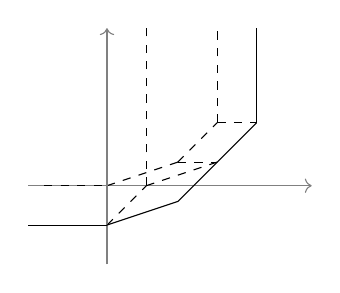
\begin{tikzpicture}
\draw[->,gray] (-1,0) -- (2.6,0);
\draw[dashed] (-0.8,0) -- (0,0);
\draw[dashed] (0,0) -- (0.9,0.3);
\draw[dashed] (0.9,0.3) -- (1.4,0.8);
\draw[dashed] (1.4,0.8) -- (1.4,2);
\draw[dashed] (-1,-0.5) -- (0,-0.5);
\draw[dashed] (0,-0.5) -- (0.5,0);
\draw[dashed] (0.5,0) -- (0.5,2);
\draw[->,gray] (0,-1) -- (0,2);
\draw[dashed] (1.4,0.8) -- (1.9,0.8);
\draw[dashed] (0.9,0.3) -- (1.4,0.3);
\draw[dashed] (0.5,0) -- (1.4,0.3);
\draw (-1,-0.5) -- (0,-0.5);
\draw (0,-0.5) -- (0.9,-0.2);
\draw (0.9,-0.2) -- (1.9,0.8);
\draw (1.9,0.8) -- (1.9,2);
\end{tikzpicture}
\end{tabular}
\end{center}

Consider the special case $P=t^a\delta^n,L=t^b \delta^m$,
then we want to show that the corresponding Newton polygons satisfies the relation in the graph:
\\
\begin{center}
\begin{tabular}{cc}
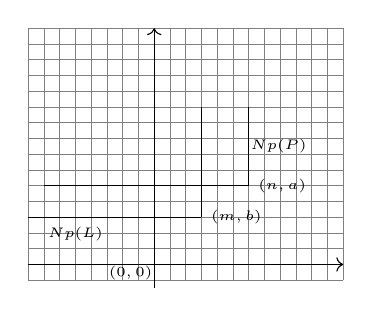
\begin{tikzpicture}
\draw[step=0.2,gray,very thin] (-1.6,-0.2) grid (2.4,3);
\draw (-1,0.6) node[anchor=north] {\tiny $Np(L)$};
\draw (1.1,1.5) node[anchor=west] {\tiny $Np(P)$};
\draw (-0.3,0.1) node[anchor=north] {\tiny $(0,0)$};
\draw[->] (-1.6,0) -- (2.4,0);
\draw (-1.6,0.6) -- (0.6,0.6) node[anchor=west] {\tiny $(m,b)$};
\draw (0.6,0.6) -- (0.6,2);
\draw (-1.4,1) -- (1.2,1) node[anchor=west] {\tiny $(n,a)$};
\draw (1.2,1) -- (1.2,2);
\draw[->] (0,-0.3) -- (0,3);
\end{tikzpicture}
&
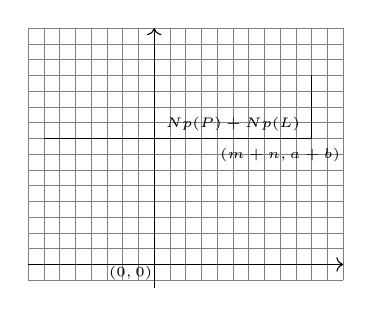
\begin{tikzpicture}
\draw[step=0.2,gray,very thin] (-1.6,-0.2) grid (2.4,3);
\draw (-1.4,1.6) -- (2,1.6);
\draw (1.6,1.6) node[anchor=north] {\tiny $(m+n,a+b)$};
\draw (-0.3,0.1) node[anchor=north] {\tiny $(0,0)$};
\draw (2,1.6) -- (2,2.4);
\draw (1,2) node[anchor=north] {\tiny $Np(P)+Np(L)$};
\draw[->] (-1.6,0) -- (2.4,0);
\draw[->] (0,-0.3) -- (0,3);
\end{tikzpicture}

\end{tabular}
\end{center}


Check that 
$$
\begin{aligned}
&\delta t^b=t^b(b+\delta)\\
&\delta^n t^b=t^b(b+\delta)^n
\end{aligned}
$$
Compute:
$$
\begin{aligned}
PL=t^a\delta^n t^b\delta^m&=t^{a+b}(b+\delta)^n\cdot\delta^m\\
&=t^{a+b}\sum^n_{k=0}\left(
\begin{array}{c}
n\\
k
\end{array}
\right)
b^{n-k}\delta^{m+k}
\end{aligned}
$$
NB. The boundary part of $PL$ is $t^{a+b}\delta^{n+m}$.They indeed satisfies the relation in the picture 1

In general:
$$
\begin{aligned}
P&=a_0 \delta^n+a_1\delta^{n-1}+...\\
L&=b_0\delta^m+b_1\delta^{m-1}+...
\end{aligned}
$$

$PL=Q+R$, where $Q$ is the principal term, while $R$ is the remainder $R>Q$
$$
Q=\sum_{
	\substack{
	\text{\tiny$(i_1,j_1)\in$}
	\\ 
	\text{\tiny boundary of $P$}
	}
	}
\sum_{
	\substack{
	\text{\tiny$(i_2,j_2)\in$}
	\\ 
	\text{\tiny boundary of $L$}
	}
	}
	a_{i_1,j_1}b_{i_2,j_2}t^{j_1+j_2}\delta^{i_1+i_2}
$$

$$
Np(Q)=Np(PL)
$$
Boundary part of $Q$
$$
\sum_{
	\substack{
	(s_1,s_2)\in\\ 
	\text{\tiny boundary of $PL$}
	}
	}
\sum_{
	\substack{
	\text{\tiny $(i_1,j_1)+(i_2,j_2)$}
	\\ 
	\text{\tiny$=(s_1,s_2)$}
	}
	}a_{i_1,j_1}b_{i_2,j_2}t^{j_1+j_2}\delta^{i_1+i_2}
$$

If $v=(s_1,s_2)$ is a vertex in the boundary of $Np(P)+Np(L)$, then $v=u+w$ for unique vertices $u$ and $w$ of $Np(P)$ and $Np(L)$ respectively.

$\Lrta$ coefficients of $t^{s_2}\delta^{s_1}$ in the boundary part of $Q$ is nonzero

$\Lrta$ $v=(s_1,s_2)\in Np(PL)$

$\Lrta$ $Np(P)+Np(L)\subseteq Np(PL)$

The reverse inclusion is easier.
\end{proof}
\end{lemma}
\begin{cor}
Let $P$ be a differential operator, suppose its $Np(P) $ is not a sum of two polygons in a nontrivial way, then $P$, then $P$ is not a product.
\end{cor}
Here, by `` can be a sum in nontrivial way'', we mean it can't be decomposed into sum of two nontrivial newton polygons
\begin{center}
\begin{tabular}{l}
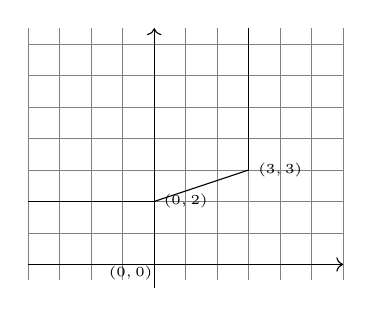
\begin{tikzpicture}
\draw[step=0.4,gray,very thin] (-1.6,-0.2) grid (2.4,3);
\draw (-0.3,0.1) node[anchor=north] {\tiny $(0,0)$};
\draw[->] (-1.6,0) -- (2.4,0);
\draw (-1.6,0.8) -- (0,0.8) node[anchor=west] {\tiny $(0,2)$};
\draw (0,0.8) -- (1.2,1.2) node[anchor=west] {\tiny $(3,3)$};
\draw (1.2,1.2) -- (1.2,3);
\draw[->] (0,-0.3) -- (0,3);
\end{tikzpicture}
\end{tabular}
\end{center}
The above polygon can not be decomposed into sum of  two nontrivial newton polygons. Its nontrivial slope is $1/3$, while polygons of degree $1$ or $2$can only have slop in $\intg$ and $\frac{1}{2}\intg$.
{\color{red} A mathematician should ask now whether the converse statement is also true}

Slope convention: Let $P\in\calk[\delta]$ be a differential operator with newton polygon $N=Np(P)$

Break points $(n_i,m_i)$
$$
0\leq n_1<n_2<n_3...<n_s=deg(P)
$$
The slopes of $P$ are
$$
\frac{m_{i+1}-m_i}{n_{i+1}-n_i}=\lambda_i
$$
and, if $n_1>0$, set $n_0:=0$

\begin{exercise}
$P$ is regular singular $\Longleftrightarrow$ $0$ is the only slope of $P$.
\end{exercise}

\begin{thm}
Let $L=\delta^n+a_1\delta^{n-1}+...+a_n$ be a differential operator and suppose
$$
Np(L)=N_1+N_2
$$
where $N_1,N_2$ are polygons with integer breakpoints and no common slopes. Then, there exist unique operators $L_1,L_2$, both monic, and 
$$
\begin{aligned}
&L=L_1L_2\\
&Np(L_1)=N_1,\ Np(L_2)=N_2.\\
\end{aligned}
$$ 
Moreover, these operators satisfy 
$$
\frakd/\frakd L\cong \frakd/\frakd L_1\oplus \frakd/\frakd L_2
$$
\begin{proof}
$(n_1,m_1),(n_2,m_2),...$ are the breakpoints of $Np(L)$

1st special case: Assume $n_1>0$, the polygon $N_1$ has only slope $0$. So $N_2$ has only slopes $>0$.
\begin{center}
\begin{tabular}{ccc}
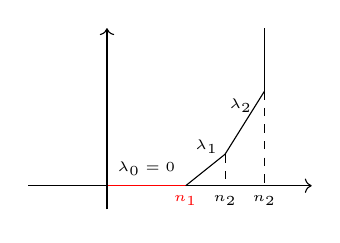
\begin{tikzpicture}
\draw[->] (-1,0) -- (2.6,0);
\draw (0.5,0) node[anchor=south] {\tiny $\lambda_0=0$};
\draw[red] (0,0) -- (1,0) node[anchor=north] {\tiny $n_1$};
\draw (1,0) -- (1.5,0.4);
\draw (1,0.5) node[anchor=west] {\tiny $\lambda_1$};
\draw (1.5,0.4) -- (2,1.2);
\draw[dashed]  (1.5,0.4) -- (1.5,0) node[anchor=north] {\tiny $n_2$};
\draw[dashed]  (2,1.2) -- (2,0) node[anchor=north] {\tiny $n_2$};
\draw (1.7,0.8) node[anchor=south] {\tiny $\lambda_2$};
\draw (2,1.2) -- (2,2);
\draw[->] (0,-0.3) -- (0,2);
\end{tikzpicture}
&
\begin{tikzpicture}
\draw[->] (-1,0) -- (2.6,0);
\draw (0.5,0) node[anchor=south] {\tiny $\lambda_0=0$};
\draw[red] (0,0) -- (1,0) node[anchor=north] {\tiny $n_1$};
\draw (1,0) -- (1,2);
\draw[->] (0,-0.3) -- (0,2);
\end{tikzpicture}
&
\begin{tikzpicture}
\draw[->] (-1,0) -- (2.6,0);
\draw (0,0) -- (0.5,0.4);
\draw (0,0.5) node[anchor=west] {\tiny $\lambda_1$};
\draw (0.5,0.4) -- (1,1.2);
\draw[dashed]  (0.5,0.4) -- (0.5,0);
\draw[dashed]  (1,1.2) -- (1,0) node[anchor=north] {\tiny $n_3-n1$};
\draw (0.7,0.8) node[anchor=south] {\tiny $\lambda_2$};
\draw (1,1.2) -- (1,2);
\draw[->] (0,-0.3) -- (0,2);
\end{tikzpicture}
\end{tabular}
\end{center}

In general, we may write $M\in \calc((t))[\delta]$ as a series
$$
M=\sum_{i>-\infty}t^i\cdot M(i)
$$
where $M(i)\in \calc[\delta]$ polynomial with bounded degree, $M(i)=0$ for $i<<0$.
Do this for $L$ and the potential $L_1, L_2$
$$
L=\sum_{i\geq m}t^i L(i)
$$
$$
L_1=\sum_{i\geq 0}t^i L_1(i)
$$
$$
L_2=\sum_{j\geq m}t^j L_2(j),
$$
where $L(k)\in\calc[\delta]$
We want $Np(L_1)=N_1$, so we ask for: 
\begin{itemize}
\item $L_1(0)=$monic of degree $n_1$
\item $deg L_1(i)<n_1$ for $i\neq 0$
\end{itemize}
$L_2(m)=$constant, since $0$ not to be slope of $L_2$. From $L\overset{!}{=}L_1L_2$ and $t^{-j}L_1(i)(\delta)t^j=L_1(i)(\delta+j)$, get
$$
\sum_{k\geq m}t^{k}\sum_{i+j=k,i \geq 0,j\geq m} L_1(i)(\delta+j)L_2(j)(\delta)=\sum_{k\geq m}t^{k}L(k)(\delta)
$$
Solve for $L_1(i),L_2(j) $ recursively.

In the case $k=m$,
$$
L_1(0)(\delta+m)L_2(m)(\delta)=L(m)(\delta)
$$
is the only possibility



>>>>>>>>>>4


Second special case: $n_1=0$, $N_1$ has only one slope, $\lambda$ and $\lambda$ is the minimal slope of $N$

Set $\lambda=\frac{b}{a}$, $b>0$, $a>0$ coprime integers. $\calk_a=\calc((t^{1/a}))\supseteq \calk=\calc((t))$, $s=t^{1/a}$, $\calk_a$ is a finite field extension of $\calk$ with degree $a$.

Set $\Delta=s^b\delta=t^{b/a}\delta$, $\Delta$ is not an operator on $\calk$ but on $\calk_a$. Consider $L$ as an element of the larger ring $\calk_a[\Delta]\supseteq \calk[\delta]$
$$
\begin{aligned}
L&=\delta^n+a_1\delta^{n-1}+...+a_n\\
&= (s^{-b}\Delta)^n+a(s^a)(s^{-b}\Delta)^{n-1}+...
\end{aligned}
$$
Set $P=s^{bn}L$. The factor $s^{-bn}$ makes $P$ unitary in $\Delta$. $P\in\calc((s))[\Delta]$. Look at the Newton polygon of $P$. It has the smallest slope $0$, thus it reduce to the first speciral case. Check this:
$$
\begin{aligned}
L&=a_{0,m_1}t^{m_1}\delta^0
+a_{n_1,m_2}t^{m_2}\delta^{n_2}+...+\text{ irrelevant terms }\\
& a_{0,m_1} s^{m_1 a}\Delta^0+a_{n_2,m_2}s^{m_2 a}(s^{-b}\Delta)^{n_2}+\text{junk}\\
&=a_{0,m_1} s^{m_1 a}\Delta^0+a_{n_2,m_2}s^{m_2 a-n_2 b}\Delta^{n_2}+\text{junk}\\
&=a_{0,m_1} s^{m_1 a}\Delta^0+a_{n_2,m_2}s^{m_1 a}\Delta^{n_2}+\text{junk}\\
\end{aligned}
$$
The last equality comes from $a(m_1-m_2)=b n_2$

\begin{tikzpicture}
\draw[->,gray] (-1,0) -- (2.6,0);
\draw (0,-0.5) node[anchor=east] {\tiny $m_1$};
\draw (0,-0.5) -- (1,-0.25);
\draw[dashed] (1,-0.25) -- (0,-0.25) node[anchor=east] {\tiny $m_2$};
\draw[dashed] (1,-0.25) -- (1,0) node[anchor=south] {\tiny $n_2$};
\draw[->,gray] (0,-1) -- (0,2);
\end{tikzpicture}
\begin{tikzpicture}
\draw[->,gray] (-1,0) -- (2.6,0);
\draw (1,-0.25) -- (0,-0.25) node[anchor=east] {\tiny $m_1 a$};
\draw[dashed] (1,-0.25) -- (1,0) node[anchor=south] {\tiny $n_2$};
\draw[->,gray] (0,-1) -- (0,2);
\end{tikzpicture}

Form 1st special case: $P=P_1P_2$ with $Np(P_1)$ only slope $0$.
$$
L=s^{-nb}P=s^{-nb}P_1P_2\overset{?}{=}L_1L_2
$$
The problem now is how to make sure that $L_i$ are infact in $\calc((t))[\delta]$ ($P_i$ are naturally in $\calc((s))[\delta]$).

Use Galois theory (descent) to show $L_i\in \calc((t)[\delta])$. (a priori in  $\calc((t^{1/a}))[\delta]$)

The Galois group $G=Gal(\calk_a/\calk)$ acts on $\calc((s))[\delta]$ by acting on coefficients. Fixed points are $\calc((t))[\delta]$, so we nned $\sigma(L_i)=L_i,\forall \sigma\in G$
$$
L=L_1L_2,\ \ \sigma L=\sigma L_1\sigma L_2
$$
$$
\sigma L=L\Lrta L=L_1L_2=\sigma L_1\sigma L_2
$$
But decomposition is unique! $Np(L_1)=Np(\sigma L_1)$ $\Lrta \sigma L_1=L_1$ and $\sigma L_2=L_2$.

\underline{symmetry} These special case also work if the smallest slope of $N$ occurs in $N_2$. Use the map
$$
\begin{aligned}
\varphi:&\calc((t))[\delta]\lrta \calc((t))[\delta]\\
& \sum a_i\delta^i\longmapsto \sum(-\delta^i)a_i
\end{aligned}
$$

Just check $\varphi(L_1L_2)=\varphi(L_2)\varphi(L_1)$ and $Np(\varphi(L))=Np(L)$.


\underline{Existence of Decomposition in general} The smallest slope $\lambda$ of $N$ belongs to $N_1$ (or to $N_2$) According to special cases $L=AB$. $A$ has only slope $\lambda$. Induction on the number of distinct slopes
$B=B_1B_2$ $Np(B_2)=N_2$
$$
L=(AB_1)B_2
$$ 
and set $L_1:=AB_1$, $L_2:=B_2$.

\underline{Unicity}: $L=L_1L_2=\tilde{L}_1\tilde{L}_2$ Suppose again the smallest slope $\lambda$ of $N$ occurs in $N_1$
$$
L_1=AB,\ \ \ A,\tilde{A} (\text{monic })
$$
$$
\tilde{L}_1=\tilde{A}\tilde{B}\text{ only slope $\lambda$ }
$$
$$
L=A(BL_2)=\tilde{A}(\tilde{B}\tilde{L}_2)
$$
unicity in the special case $\Lrta A=\tilde{A}$

Induction on degrees $\Lrta  B=\tilde{B}$ and hence $L_1=\tilde{L}_1$ and $L_2=\tilde{L}_2$

\underline{additional statement}
Have short exact sequence:
Want a>>>>>>>

or show $\Psi$ is an isomorphism
\[
\begin{tikzcd}
0\arrow[r]  & \frakd/\frakd L_1  \arrow[r,"L_2"] & \frakd/\frakd L\arrow[r] \arrow[d,equal] & \frakd/\frakd L_2\arrow[r,"\pi"]  & 0 \\
0\arrow[r]  & \frakd/\frakd \tilde{L}_2\ar[rru,"\Psi"]  \arrow[r,"\tilde{L}_1"] & \frakd/\frakd L\arrow[r,"\pi"] & \frakd/\frakd \tilde{L}_1\arrow[r]  & 0 
\end{tikzcd}
\]
We have $N=N_1+N_2=N_2+N_1$ get 
$$
L+\tilde{L}_2\tilde{L}_1
$$
unique with $Np(\tilde{L}_i)=N_i$
Claim is an isomorphism:
$dim \frakd/\frakd \tilde{L}_2=dim \frakd/\frakd L_2=deg L_2=deg\tilde{L}_2=d$.
It suffices to show $\Psi$ is injective. Pick $A\in\frakd,deg(A)< d, A\neq 0$. Suppose $\Psi(\text{Class of $A$})=0$ $A\tilde{L}_1B L_2$ for some $B\in \frakd$ $\tilde{L}_1$ and $L_2$ have no common slopes $\Lrta Np(L_2)\subseteq Np(A)\Lrta deg(L_2)=d\geq deg(A)< d$, Then $\Psi$ is injective.
\end{proof}

\begin{ex}
$L=\delta^2+(\frac{1}{t^2}+\frac{1}{t})\delta+(\frac{1}{t^3}-\frac{2}{t^2})$.

Factorize $L$, $s=t,\Delta=t\delta$.

We use the identity $\delta62=t^{-2}\Delta^2-t^{-1}\Delta$

$$
\begin{aligned}
L&=\delta^2+(t^{-2}+t^{-1})\delta+(t^{-3}+2t^{-2})\\
&=t^{-2}\Delta^2+(t^{-3}+t^{-2}-t^{-1})\Delta+(t^{-3}-2t^{-2})\\
&=\Delta^2+(t^{-1}+1-t)\Delta+(t^{-1}-2)\\
&\ \\
P&=\Delta^2+(t^{-1}+1-t)\Delta
+(t^{-1}-2)
\end{aligned}
$$
\end{ex}


\end{thm}




\end{document}
